\openingarticle
\def\ppages{\pagerange{Forssman:firstpage}{Forssman:lastpage}}
\def\shorttitle{Late Holocine Rockshelter, Botswana}
\def\maintitle{The Late Holocene Occupation of Mafunyane Shelter, Eastern Botswana}
\def\shortauthor{Tim Forssman}
\def\authormail{tim.forssman@gmail.com}
\def\affiliation{Postdoctoral Researcher at the Rock Art Research Institute, School of Geography, Archaeology and Environmental Studies, University of the Witwatersrand (South Africa)}
\def\thanknote{\footnote{This paper is the product of DPhil research carried out at the University of Oxford (UK)}}
%--------------------------------------------------------------
\mychapter{\maintitle}
\begin{center}
	{\Large\scshape\shortauthor \thanknote}\\[1em]
	\email \\
	\affiliation
\end{center}
\vspace{3em}
\midarticle
%--------------------------------------------------------------
\label{Forssman:firstpage}

%----------------------------------------------------------------------------------------
	%----------------------------------------------------------------------------------------
	%	ABSTRACT
	%----------------------------------------------------------------------------------------
\begin{myabstract}
		\noindent  Mafunyane \marginnote{Abstract} Shelter is a small rockshelter situated in eastern Botswana along the Limpopo River. The site was occupied from possibly the first centuries \AD until the Leopard’s Kopje period, \AD 1000 to 1300. 
		Excavations revealed an extensive Later Stone Age (LSA) assemblage including stone tools, beads and a diverse faunal record as well as ceramics, a figurine fragment and various metal and metal-working associated finds. Inside the rockshelter is a limited number of rock markings including paintings, cupules and grooves. The site was originally excavated by \parencite{Walker_1994} but until now has not been dated. Here, new findings from a subsequent excavation are presented along with a revised chronological sequence. 
		The occupation of Mafunyane is discussed and the implications relating to the farmer-associated items such as the ceramics and metal assemblage are considered. The results suggest that an expansion of our research approach might reveal aspects of the LSA seldom occurring at large rockshelter sites, such as specific site utilisation patterns, specialist or craft activities, and the variable social responses from forager-farmer interactions.
		
\keywords[Keywords]{Later Stone Age, stone tools, hunter-gatherers, forager-farmer interactions, Greater Mapungubwe Landscape, eastern Botswana}
	\end{myabstract}

	
	%\section{Introduction}
	\lettrine[nindent=0em,lines=3]{T}{he} Later Stone Age (LSA) sequence of the Greater Mapungubwe Landscape, which includes parts of eastern Botswana, northern South Africa and south-western Zimbabwe (\cref{fig:Forssman-Figure01}), has been at the centre of a number of studies \parencites[e.g.][]{Hall_2000}{vanDoornum_2005}{vanDoornum_2007}{vanDoornum_2008}{vanDoornum_2014}{Forssman_2010}{Forssman_2013a}{Forssman_2013b}{Forssman_2013c}{Forssman_2014a}{Forssman_2014b}. 
Most have been restricted to large rockshelter sites in South Africa, and from this work a fairly comprehensive occupation sequence has been established. In an attempt to expand upon this, the author conducted research in eastern Botswana where a series of sites including open-air camps, small or discrete rockshelters and homesteads containing LSA stone artefacts were excavated. The aim of this study was to develop a regional understanding of the local LSA sequence and perform trans-national research, crossing modern boundaries that may not have been present in the past but which potentially confine our work today \parencites[for details see][]{Forssman_2013c}{Forssman_2014a}{Forssman_2014b}{Forssman_2015}. One of the excavated sites, Mafunyane Shelter, is a small rockshelter originally excavated by \textcite{Walker_1994} as Tuli Lodge. 
In new excavations at the site an archaeological assemblage was uncovered that offered an additional perspective on landscape patterns, forager-farmer interactions and metal-working. Presented here are these results.
	
\begin{figure}
		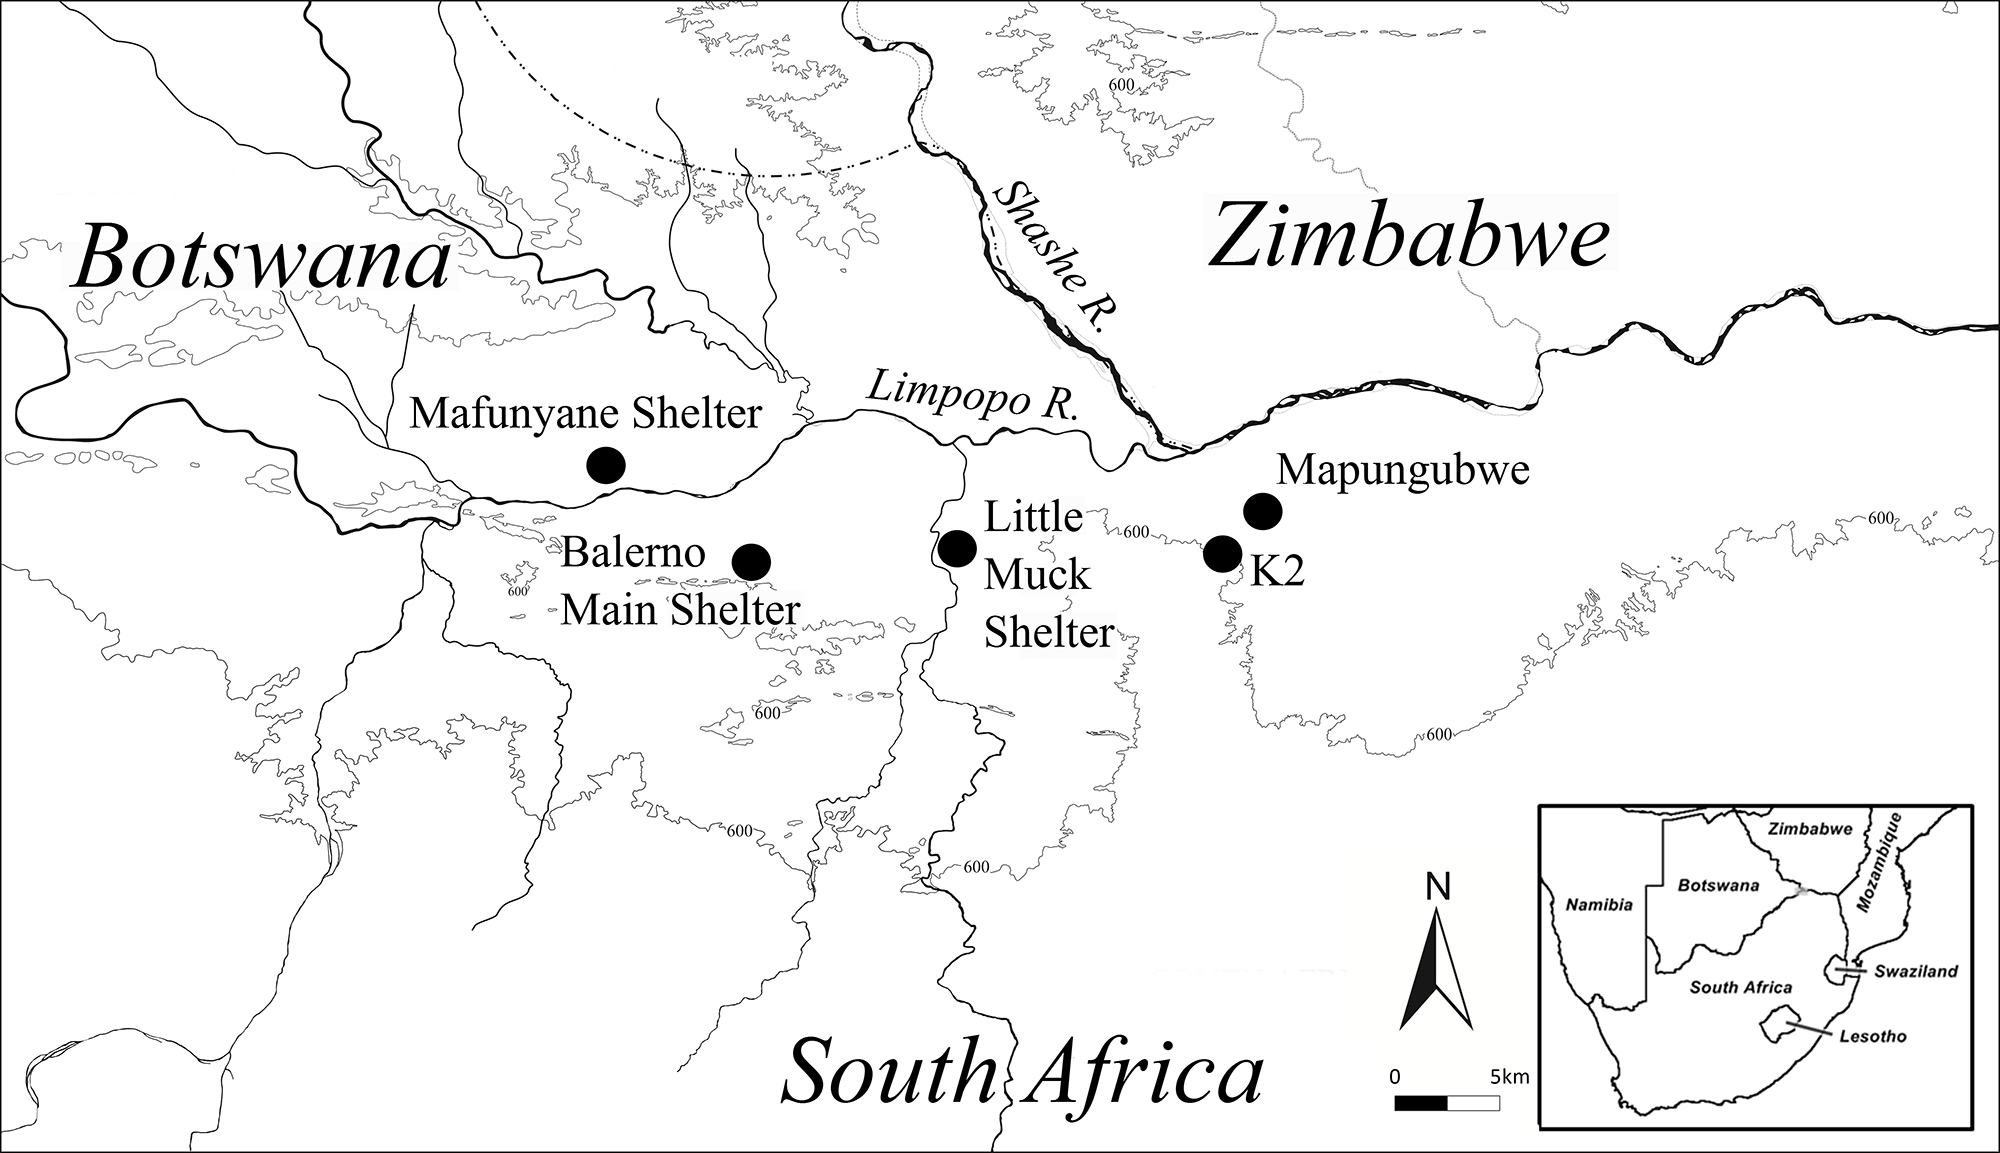
\includegraphics[width=\linewidth]{figures/Forssman-Figure01}
		\caption{The Greater Mapungubwe Landscape with sites mentioned in the text and other prominent sites.}
		\label{fig:Forssman-Figure01}
\end{figure}
	
%	\section*{Mafunyane Shelter}	
	Mafunyane \marginnote{Mafunyane Shelter} is situated in a sandstone belt that stretches along the Motloutse, Limpopo, and Shashe Rivers. Within this area are low-lying koppies (sandstone inselbergs) and ridges interspersed with water networks and small floodplains. The area immediately surrounding the site is characterised by a fine loam to clay soil horizon, created by depositional processes from flooding by the Limpopo River, \SI{460}{\meter} away, and a nearby seasonal stream. 
	The vegetation around the site is characterised by dense pockets of mopane veld (\emph{Colophospermum mopane}) and more widespread vachellia and acacia open shrubland. The site’s near proximity to the Limpopo River suggests that in the past the immediate area may have been a riverine woodland, which today is restricted to the banks of major rivers due to the receding water table \parencite{Alexander_1984}.
	
	\textcite{Walker_1994} previously excavated the site under the name Tuli Lodge. It was not known at first whether Mafunyane was the \textcite{Walker_1994} site because no GPS co-ordinates were published and at the time of this study the reserve management had not been informed of his research on the farm. Once it was established that the sites were the same it was decided to re-excavate the rockshelter in order to increase the site’s sample size, obtain charcoal samples for radiocarbon dating and relate the findings made here to the broader regional sequence. \textcite{Walker_1994} revealed an extensive LSA assemblage including \num{14379} stone tools along with 21 pieces of worked bone, fragments from tortoise and ostrich eggshell bowls and containers, 67 ostrich eggshell beads, 64 potsherds, a pipe and crucible, six glass trade beads and 16 metal implements as well as large amounts of metal prills. 
	He concluded that based on the prevalence of scrapers in the assemblage, the site was occupied quite late, probably from the first few centuries\AD, and that the foragers using the site were in contact with farmers. 
In addition, he states that the rockshelter was \enquote{clearly a major living site} that 
	\enquote{was probably seasonally occupied, but it was later used by metalworking people to smelt copper} \parencite[10]{Walker_1994}. 
	
%\section*{Excavation, Stratigraphy, and Chronology}
The site’s floor was \marginnote{Excavation, Stratigraphy, and Chronology} divided into a grid of \SIrange{1}{1}{\meter} squares with alphabetical designations running east to west and numeric designations running south to north. 
Square 3C was selected for excavations primarily because it was located in an area most likely to contain a deep and intact deposit (\cref{fig:Forssman-Figure02}). 
On excavating the square it was found that a portion of it, the southwestern quadrant, protruded into what appeared to be the \textcite{Walker_1994} excavation and so this quadrant was excluded; 
thus only three quadrants were excavated to bedrock. Initially excavations were also to be conducted in the large open-air living area north of the site, but this area was found to contain little deposit and appeared highly disturbed. 
Excavations therefore only proceeded inside the rockshelter and were conducted in spits of \SI{30}{\milli\meter} following natural stratigraphic units.

	\begin{figure}
		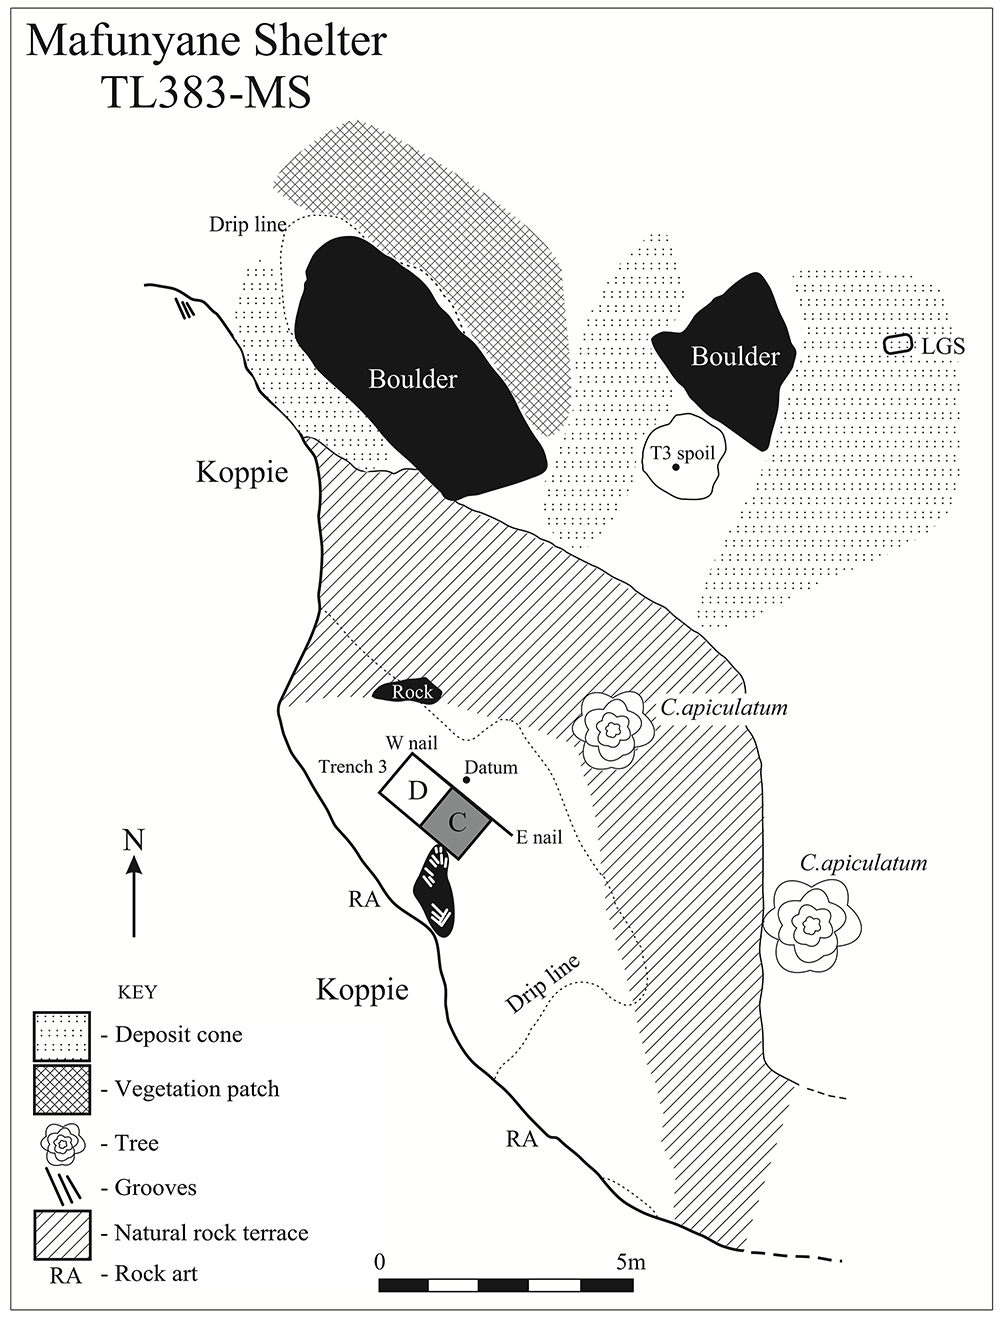
\includegraphics[width=\linewidth]{figures/Forssman-Figure02}
		\caption{Only Square C was excavated at Mafunyane since Square D protruded into the \textcite{Walker_1994} excavation, not visible on the surface but recorded once the surface layer was removed \parencite[from][96]{Forssman_2014a}.}
		\label{fig:Forssman-Figure02}
	\end{figure}

In total seven spits between the surface and bedrock were excavated, revealing three stratigraphic layers, each distinct from the other and similar to \textcite{Walker_1994}. 
The upper most layer, Pale brown sand (PBS), contains small (<\SI{25}{\milli\meter}) sandstone pebbles in an unconsolidated deposit,
 less than \SI{6}{\centi\meter} thick filling \num{2,3} buckets (\SI{13}{\liter} each). 
PBS occurred in Spit I-III but from Spit II, Ashy sand (AS) appears and may be a hearth layer. 
This layer is ash grey, loosely consolidated, with few to no pebbles and is also about \SI{6}{\centi\meter} in thickness (\num{3.4} buckets). 
The lowermost layer, Stony-ashy sand (SAS), is the most substantial (± \SI{12}{\centi\meter} in thickness; \num{4.5} buckets) and also appears to be a hearth with a similar colour to AS but with considerably more pebbles and stones included in the deposit (\cref{fig:Forssman-Figure03}); 
the depth of bedrock was on average \SI{20}{\centi\meter} below the surface and a total of \num{10.3} buckets was removed from the site \parencite[for more details see][95]{Forssman_2014a}. 

	\begin{figure}
		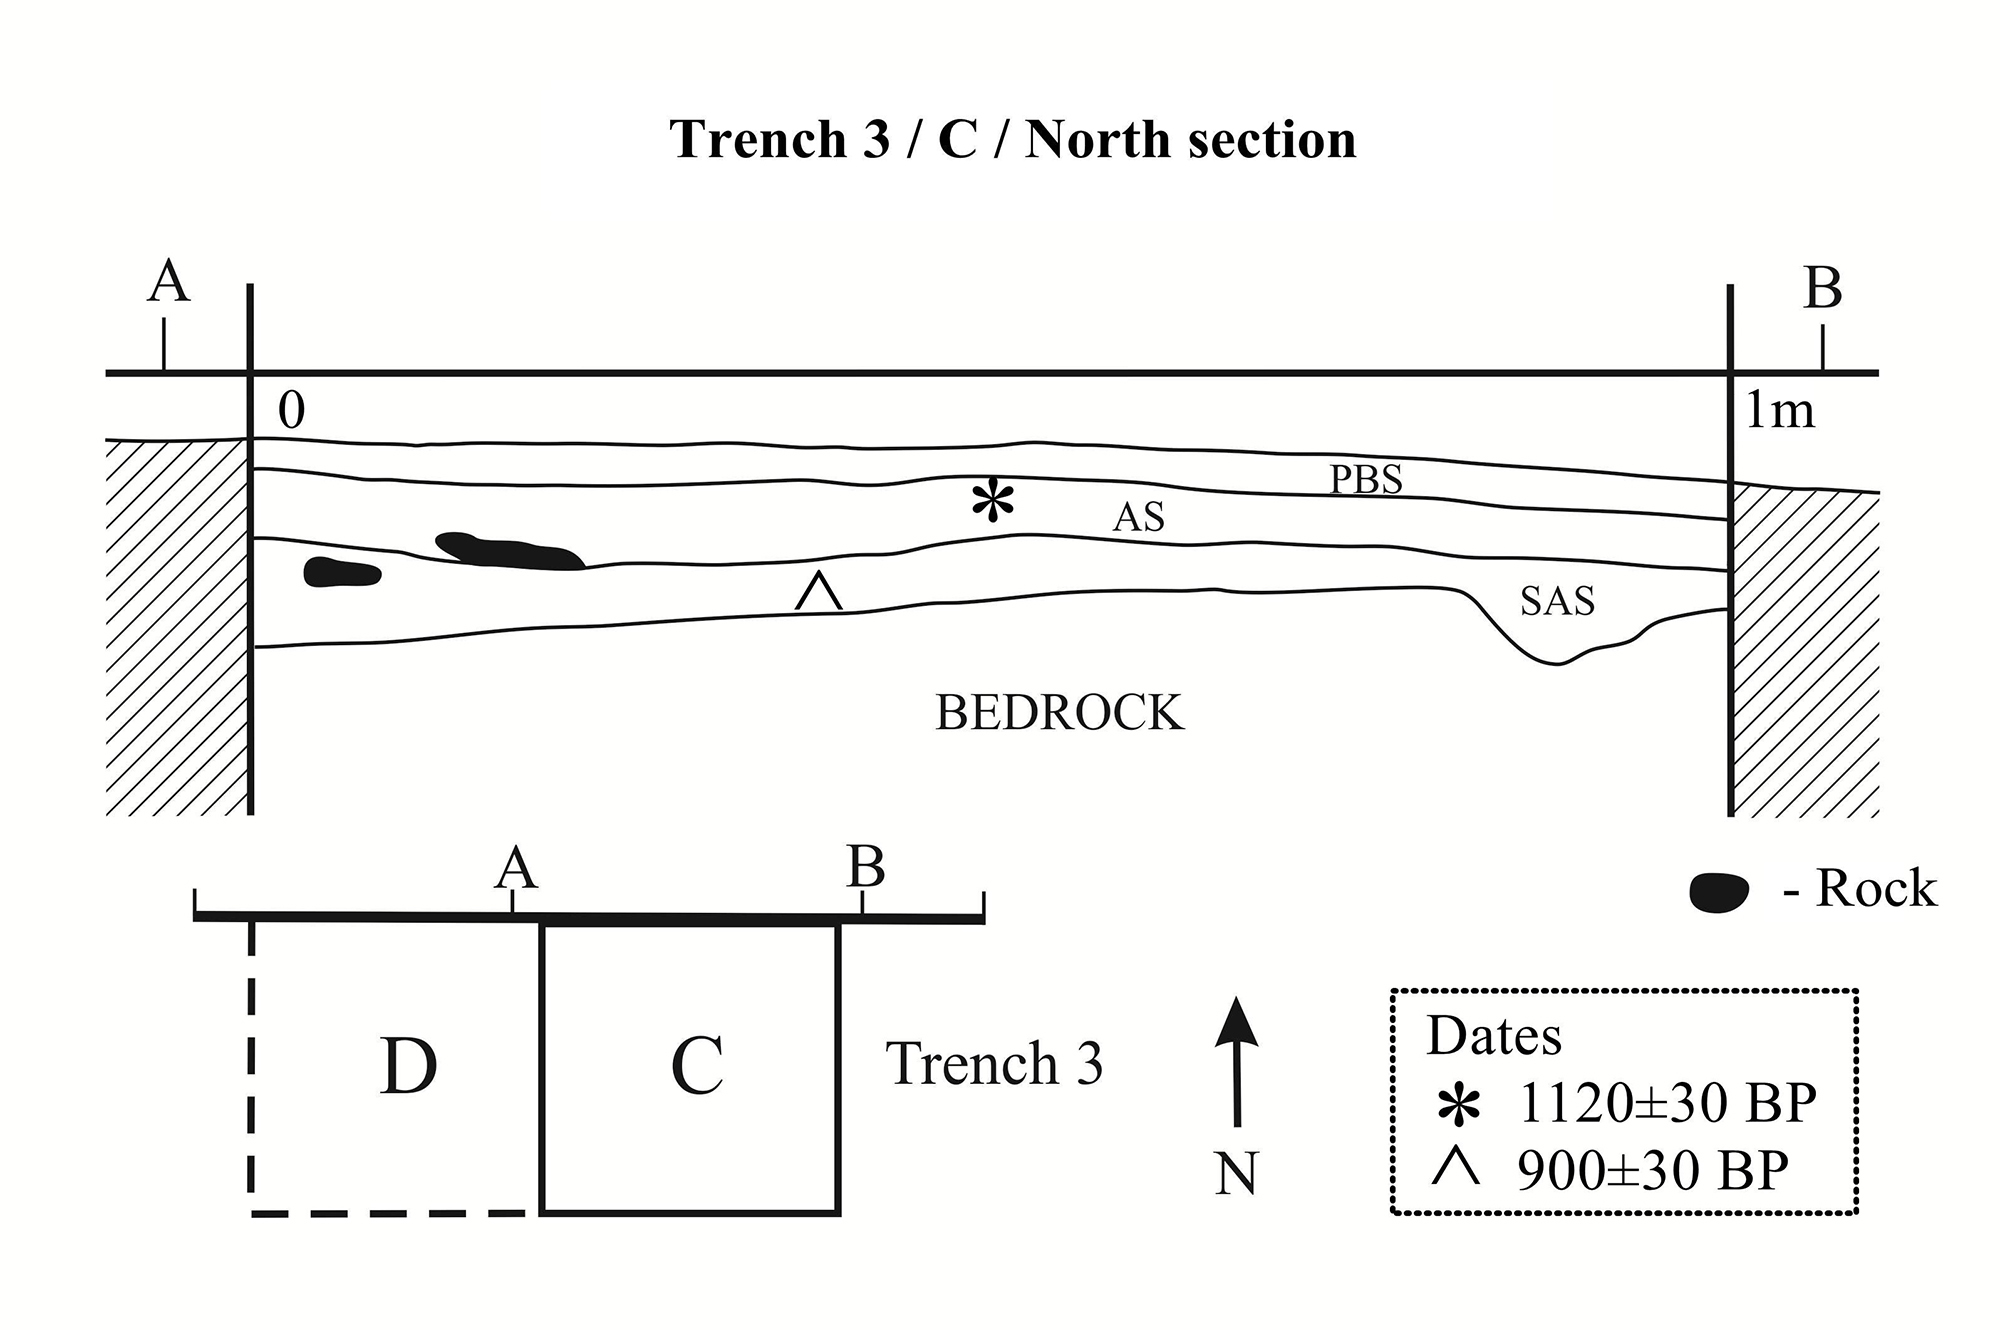
\includegraphics[width=\linewidth]{figures/Forssman-Figure03}
		\caption{Section drawing of the north wall in Square C at Mafunyane indicating the approximate location of the radiocarbon dates.}
		\centering
		\label{fig:Forssman-Figure03}
	\end{figure}

Two charcoal samples were submitted for radiocarbon dating to Beta Analytic and the results are presented in \cref{fig:Forssman-Table01}. 
The samples indicate that the site was occupied between \AD 941 and 1265. 
However, the more recent date is from Spit VII and the older from Spit II. 
The laboratory did not find any evidence indicating that the samples were possibly contaminated and so this does not seem to have caused the inverted dates. 
It is possible that the sample from Spit VII is ‘old wood’, which introduces an unresolvable variable into the calibration process \parencite{Kennett_2002}, but could equally have moved after deposition, possibly due to bioturbation \parencite[see][]{Lancaster_2003} or root action in the deposit (roots were recorded above bedrock). 
Ceramics do little to assist, although they appear to be contemporaneous (discussed below), and no other chronological markers were identified in the relevant spits. Therefore, the integrity of the deposit is uncertain (but see discussion below).

	\begin{figure} %TABLE 1
		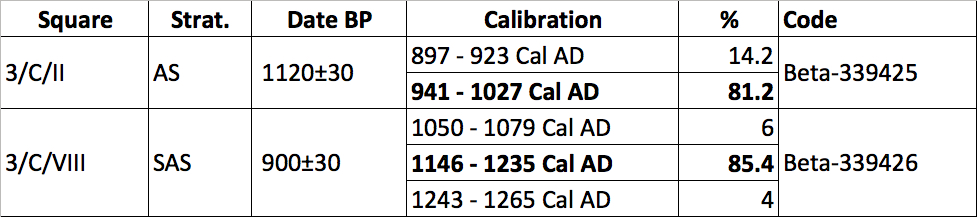
\includegraphics[width=\linewidth]{figures/Forssman-Table01}
		\captionof{table}{Calibrated radiocarbon dates on charcoal samples from Mafunyane.}
		\label{fig:Forssman-Table01}
	\end{figure}

%\section*{The Stone Tool Assemblage}

Square C \marginnote{The Stone Tool Assemblage} produced a total of \num{6349} stone tools within \num{10.3} buckets (\SI{0.1}{\meter\cubed}). 
As with other rockshelter excavations in the area, the assemblage is dominated by crypto-crystalline silicates (CCS), 
after which quartz follows and then consistently low frequencies of quartzite, agate and dolerite. 
The greatest number of stone artefacts is found between Spits II and V (\cref{fig:Forssman-Figure04}), 
followed by a decrease until bedrock is reached in Spit VII (\cref{fig:Forssman-Table02}). 
A similar pattern was noted with regard to the stone tool density (artefacts/13l bucket) with the exception of the high density on the surface and in Spit I. 
If the high density of stone tools on the surface represents a forager use of the rockshelter, it may be after \AD 1200 based on the radiocarbon dates and the Leopard’s Kopje ceramics found by \textcite{Walker_1994} in the upper levels of his excavation. 

	\begin{figure} %Figure 4
		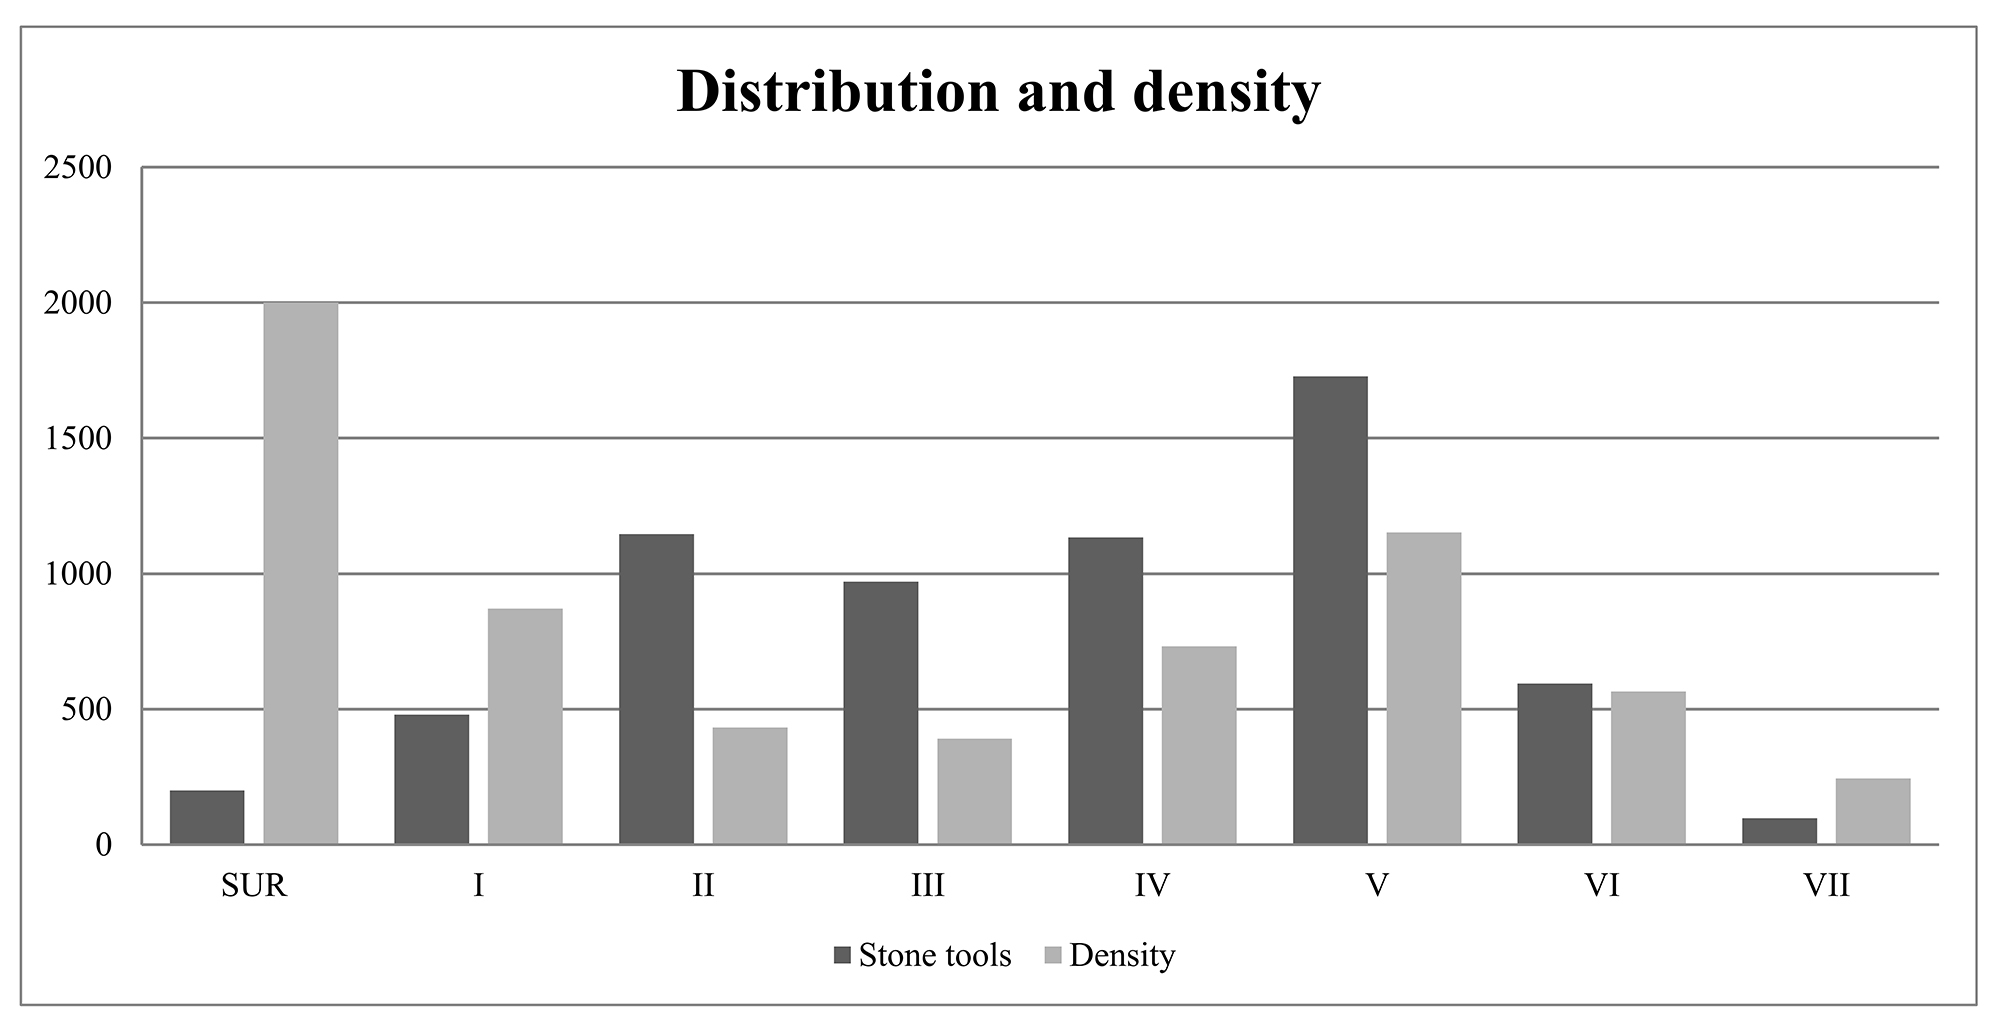
\includegraphics[width=\linewidth]{figures/Forssman-Figure04}
		\caption{The distribution and density (artefacts/\SI{13}{\liter} bucket) of stone tools at Mafunyane.}
		\label{fig:Forssman-Figure04}
	\end{figure}

	\begin{figure} %TABLE 2
		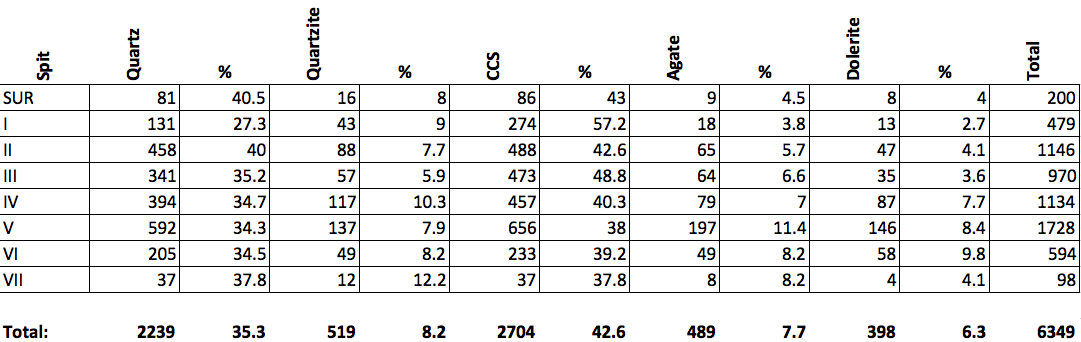
\includegraphics[width=\linewidth]{figures/Forssman-Table02}
		\captionof{table}{Raw material use through the spits and total stone tool distribution.}
		\label{fig:Forssman-Table02}
	\end{figure}

Below the stone tool assemblage has been separated into two categories based on the \textcite{Walker_1994} typological breakdown: 1) debitage and utilised pieces and 2) formal tools.

%\subsection*{Debitage and utilised pieces}
Debitage are \marginnote{Debitage and utilised pieces} pieces that might have been used but do not contain secondary working. 
At Mafunyane, this amounts to \SI{98.3}{\percent} of the rockshelter’s total stone tool assemblage (n=\num{6242}). 
The majority of these are chips, comprising of \num{3391} artefacts and \SI{53.4}{\percent} of the total assemblage. 
Chips measure less than \SI{10}{\milli\meter}
  in length and do not contain secondary working or high utilisation damage \parencite[see][]{Deacon_1984a}. 
 The presence of chips indicates that a) the deposit has not been exposed to high levels of colluvial action \parencite{Kuman_2009} and b) primary stone tool knapping occurred at the site.

There are 82 cores (\SI{1.3}{\percent}) and most were found in Spits IV and V, part of SAS, totalling 52 artefacts and \SI{63.4}{\percent} of the core category. 
Irregular cores are the most frequent core type (n=37). 
This is followed by single platform and rice seed (n=10 each), casual (n=9), preliminary flaked (n=8), bipolar bladelet (n=3), radial (n=2) and bipolar, bipolar radial and opposed platform cores (n=1 each). 
The bipolar, radial and rice seed cores indicate that a bipolar flaking technique was used \parencite[see][]{vanDoornum_2005}
 and total 15 artefacts. 
 \textcite[259]{vanDoornum_2008} found that at Balerno Main Shelter bipolar flaking increased from the beginning of contact with farming (agropastoralist) communities in the first centuries\AD. 
 It is not possible to draw the same conclusion at Mafunyane since the site appears to have been occupied for only a short phase within this period.
 
 %/subsection*{Formal Tools}
 The formal tool assemblage, which totals 107 \marginnote{Formal Tools} artefacts (\SI{1.7}{\percent}), 
is not unlike other LSA assemblages in the area \parencite{vanDoornum_2005}(\cref{fig:Forssman-Figure05}). 
Most of the formal tools were produced using CCS materials (\cref{fig:Forssman-Figure06})
  and were found in Spits IV and V, after which they decrease until bedrock is reached in Spit VII. Stratigraphically it is the lowermost unit, SAS, that contains the majority of the formal tools (n=79; \SI{73.8}{\percent}). 
  Scraping tools (\SI{57}{\percent}), of which there are 11 different forms,
   dominate the formal tool assemblage and fall into three size classes: 
   small (<\SI{20}{\milli\meter}; n=51; \SI{83.6}{\percent}), 
   medium (\SIrange{20}{30}{\milli\meter}; n=6; \SI{9.8}{\percent}) and large (>\SI{30}{\milli\meter}; n=4; \SI{6.6}{\percent}; 
   \cref{fig:Forssman-Table03}). 
 Also frequent are backed stone tools (\SI{25.2}{\percent}), a category which includes segments in various stages of completion (n=12), 
whole (n=10) and broken (n=1) segmented backed bladelets and two broken and one complete backed bladelet. 
The only other tools found at Mafunyane were adzes (n=5) possibly used for woodworking \parencite{Walker_1994}, awls (n=2) associated with boring activities \parencite{Deacon_1984a}, and miscellaneous backed pieces (MBP; n=11). 
   
	\begin{figure} %Figure 5
		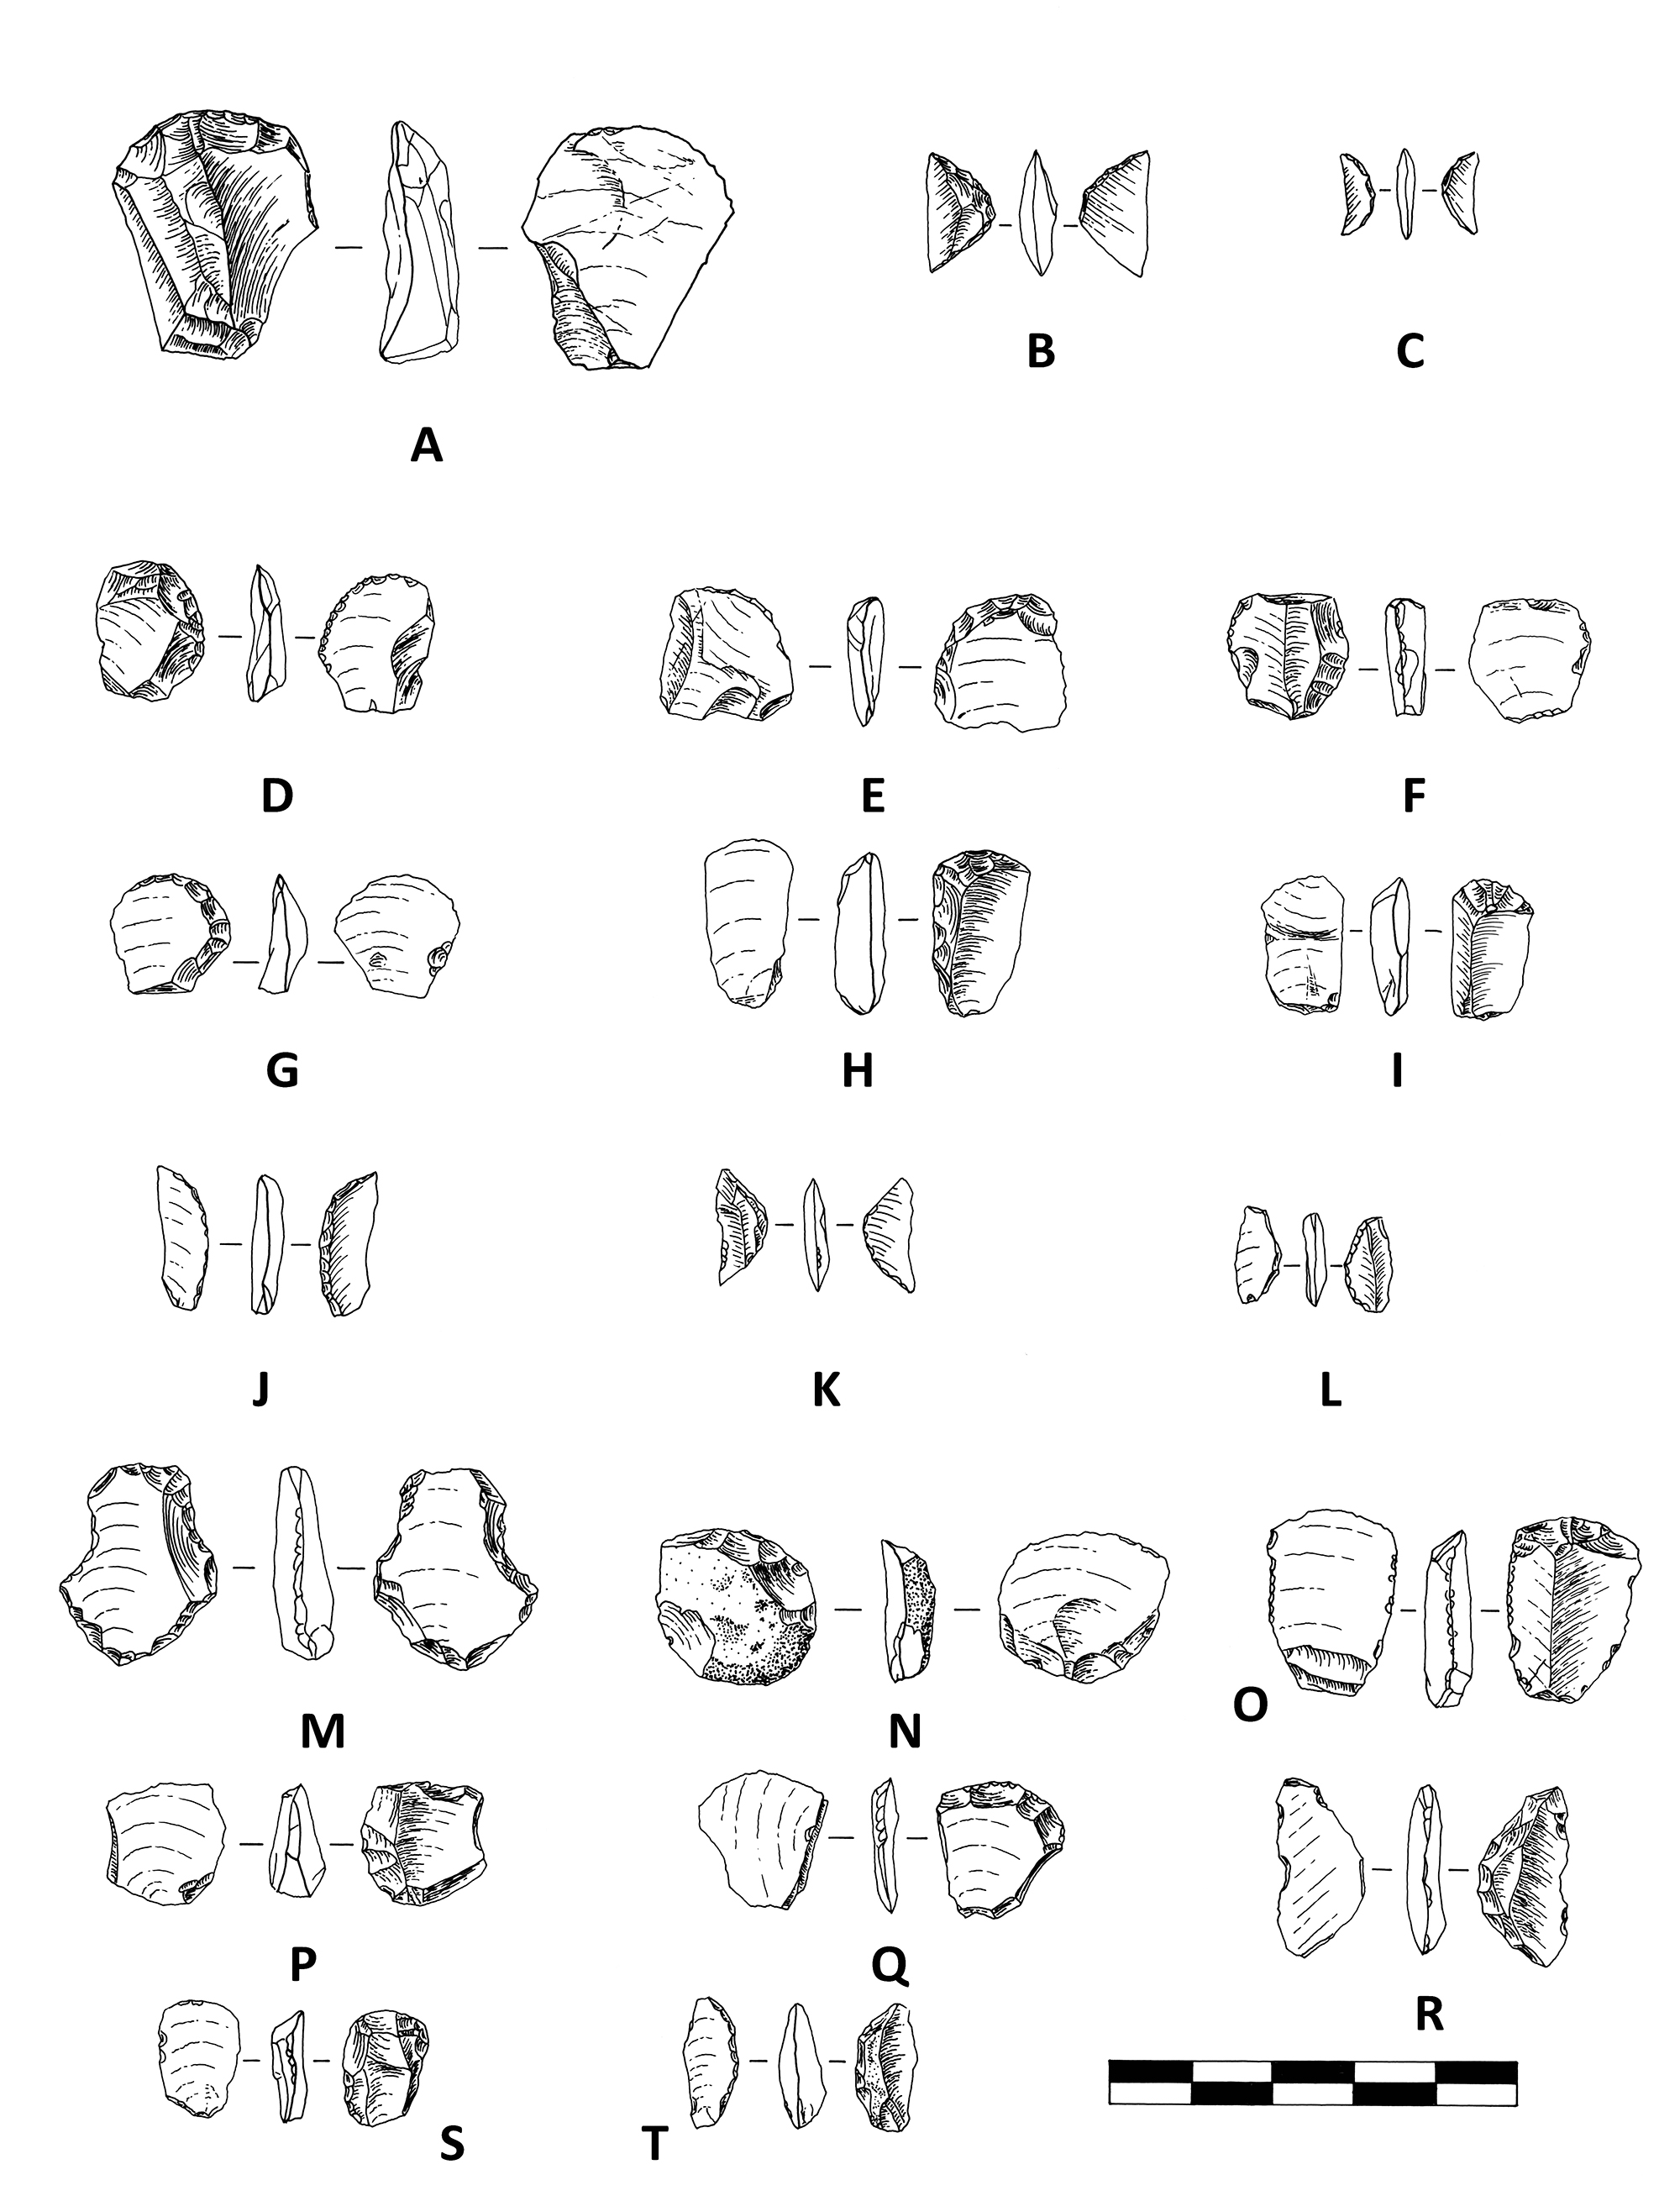
\includegraphics[width=\linewidth]{figures/Forssman-Figure05}
		\caption{Examples of formal tools from Mafunyane: A \& O, medium end scarper; B, C, K \& R, segment; D, F \& S, small side scraper; E, G-I, N, P \& Q, small end scraper; J, L \& T, segmented backed bladelet; and M, adze.}
		\label{fig:Forssman-Figure05}
	\end{figure}
	
		\begin{figure} %Figure 6
			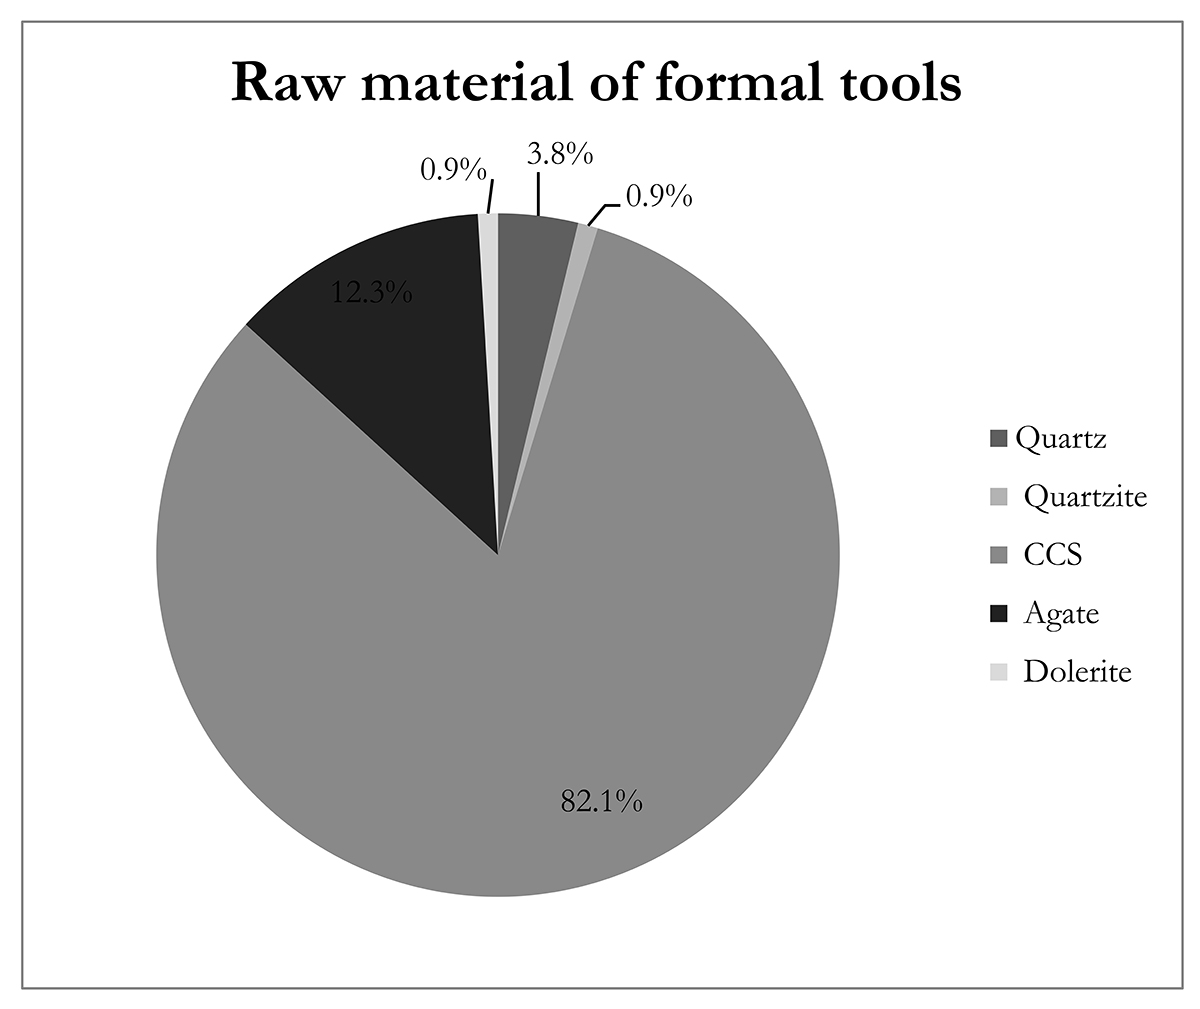
\includegraphics[width=\linewidth]{figures/Forssman-Figure06}
			\caption{Raw material utilisation in the formal tool assemblage.}
			\label{fig:Forssman-Figure06}
		\end{figure}
	
	\begin{figure} %TABLE 3
		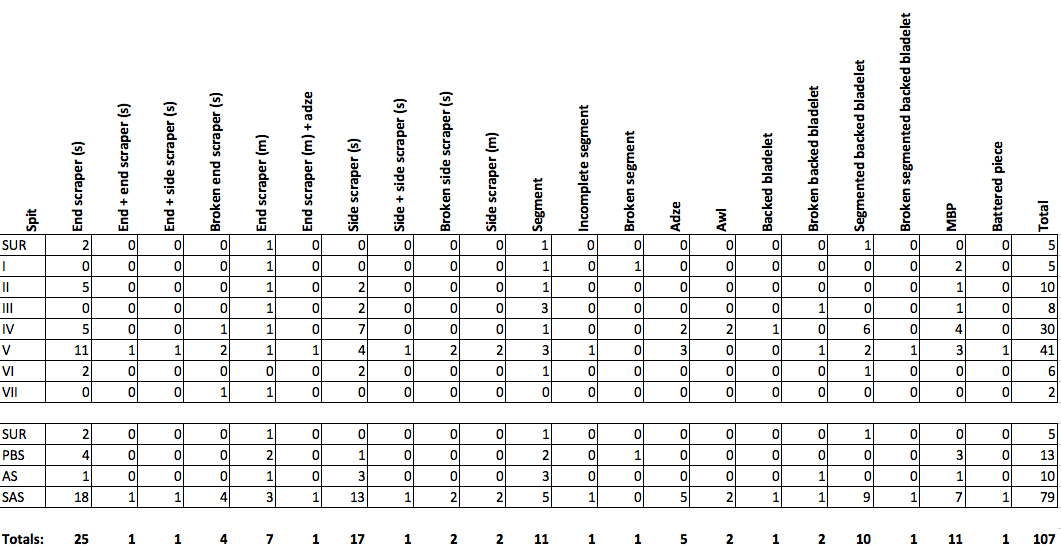
\includegraphics[width=\linewidth]{figures/Forssman-Table03}
		\captionof{table}{Formal tool types and distribution separated by spits and stratigraphic layers. Scrapers marked with s (small), m (medium) and l (large) indicate their size class.}
		\label{fig:Forssman-Table03}
	\end{figure}
   
   The majority of scrapers (n=46) and backed tools (n=18) were found in SAS, the lowermost unit (\cref{fig:Forssman-Table04}). 
  It is also within this stratigraphic unit that the majority of stone tools were found and may be a period of increased activity or in the population living at the rockshelter (but no depositional study has been performed). Scraper and backed tool lengths varied between the spits and throughout the deposit. The average scraper length is \SI{16.3}{\milli\meter} 
   while the average length of backed tools is \SI{14.7}{\milli\meter}. 
  It is clear that while scraper lengths vary from the base of the trench to the surface, there is no distinctive pattern, 
   although in general they appear to increase in size across the spits whereas between the stratigraphic units they decrease. Backed tools on the other hand decrease in size between both the spits and stratigraphic units. These findings are consistent with those made by \textcite[31]{Walker_1994}.
   
   	\begin{figure} %TABLE 4
   		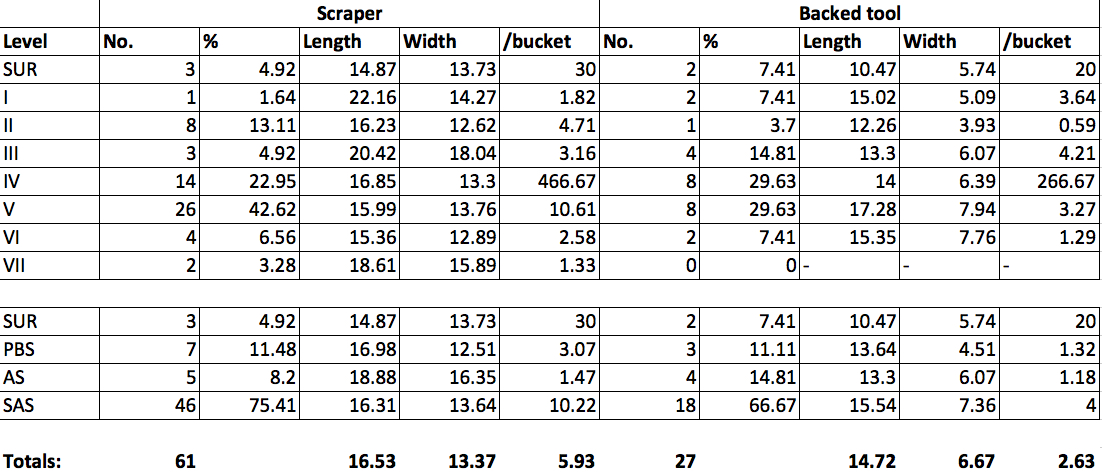
\includegraphics[width=.8\linewidth]{figures/Forssman-Table04}
   		\captionof{table}{Scraper and backed stone tool distribution and density based on the spits (above) and stratigraphic layers (below).}
   		\centering
   		\label{fig:Forssman-Table04}
   	\end{figure}
   
%\section*{Ceramics}

Ceramics occur from the \marginnote{Ceramics} surface to Spit VI but generally in low densities (on average 3/bucket; \cref{fig:Forssman-Figure07}). 
A total of 31 sherds were recovered with most being undiagnostic or plain 
(n=28; \SI{90.3}{\percent}). 
Two decorated (\SI{6.5}{\percent}) and one plain rim (\SI{3.2}{\percent}) was also found as well as a decorated rim found on the surface outside the excavation but still within the rockshelter (\cref{fig:Forssman-Figure08}). 
Unfortunately, the decorated sherds are small and difficult to place within a ceramic facies with any certainty. However, based on the incised decorations and their location in the neck it is possible that they are from the K2 facies.\footnote{\AD 1000 to 1220; ceramic identification Antonites pers. comm. 2015} 
This designation is supported by the Leopard’s Kopje ceramics (\AD 1000 to 1300; K2 is a sub-group within the Leopard’s Kopje branch) identified by \textcite{Walker_1994}. 
If accurate, the ceramic facies represented at the site overlaps with a large portion of the radiocarbon dates from \AD 941 to 1265.

	\begin{figure} %Figure 7
		\includegraphics[width=\linewidth]{figures/Forssman-Figure07}
		\caption{Ceramic distribution showing a peak in Spits II and III.}
		\label{fig:Forssman-Figure07}
	\end{figure}
	
		\begin{figure} %Figure 8
			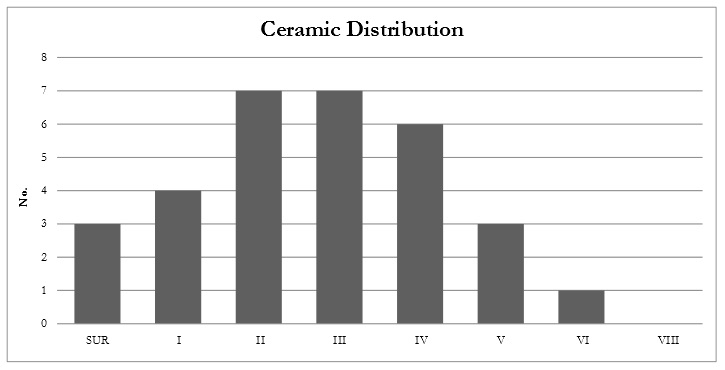
\includegraphics[width=\linewidth]{figures/Forssman-Figure08}
			\caption{Decorated ceramics from Mafunyane too small to identify with certainty but might be K2}
			\label{fig:Forssman-Figure08}
		\end{figure}

%\section*{Shell, Bone, Glass, and Metal Beads}

A total of 54 \marginnote{Shell, Bone, Glass, and Metal Beads} beads were recovered from the excavation, of which 41 are made from ostrich eggshell (\SI{75.9}{\percent}), 
six from bone (\SI{11.1}{\percent}), 
three each from land snail and glass (\SI{5.6}{\percent}) and one from metal (\SI{1.9}{\percent}; 0.1/bucket; \cref{fig:Forssman-Table05}). Ostrich eggshell beads are divided into four categories \parencite[after][]{Orton_2008}: 
complete (\SI{40}{\percent}), broken (\SI{15}{\percent}), 
incomplete/preform (\SI{15}{\percent}) and broken preform (\SI{30}{\percent}). 
All ostrich eggshell beads were measured and the complete specimens have an average length of 
\SI{3.7}{\milli\meter} and a width of \SI{3.6}{\milli\meter}. 
Of the complete beads, there are 14 small beads (< \SI{5}{\milli\meter}), 
typically associated with foragers \parencite[c.f.][]{Orton_2014}, and four medium beads (\SIrange{5}{6}{\milli\meter}). 
In both the spit and stratigraphic units the average length of beads decreased from Spit V to the surface (no complete beads were found in Spits VI and VII). 
Broken and preform ostrich eggshell bead lengths displayed no pattern but broken preforms decrease in length from the base of the trench; it might indicate that a preference for smaller beads occurred in the more recent deposits but if so one would expect the same pattern in the previous two categories. The different bead variations appear throughout the trench, barring in Spit VII,
 and no pattern is discernible (\cref{fig:Forssman-Figure09,fig:Forssman-Figure10}). 
 The presence of beads in various states of manufacture indicate that during Mafunyane’s occupation ostrich eggshell bead processing was occurring at the site, 
 and if the beads \textcite{Walker_1994} identified are included (n=67) it is possible that the manufacturing operation was either of a considerable scale or took place over a short intense period of production. 
 
    	\begin{figure} %TABLE 5
    		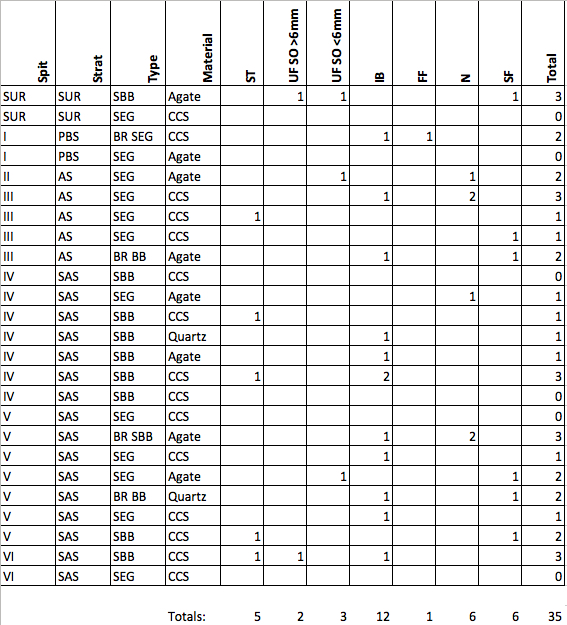
\includegraphics[width=.8\linewidth]{figures/Forssman-Table05}
    		\captionof{table}{The distribution and density of bead types from Mafunyane’s spits (above) and stratigraphic units (below).}
    		\centering
    		\label{fig:Forssman-Table05}
    	\end{figure}
 
 	\begin{figure} %Figure 9
 		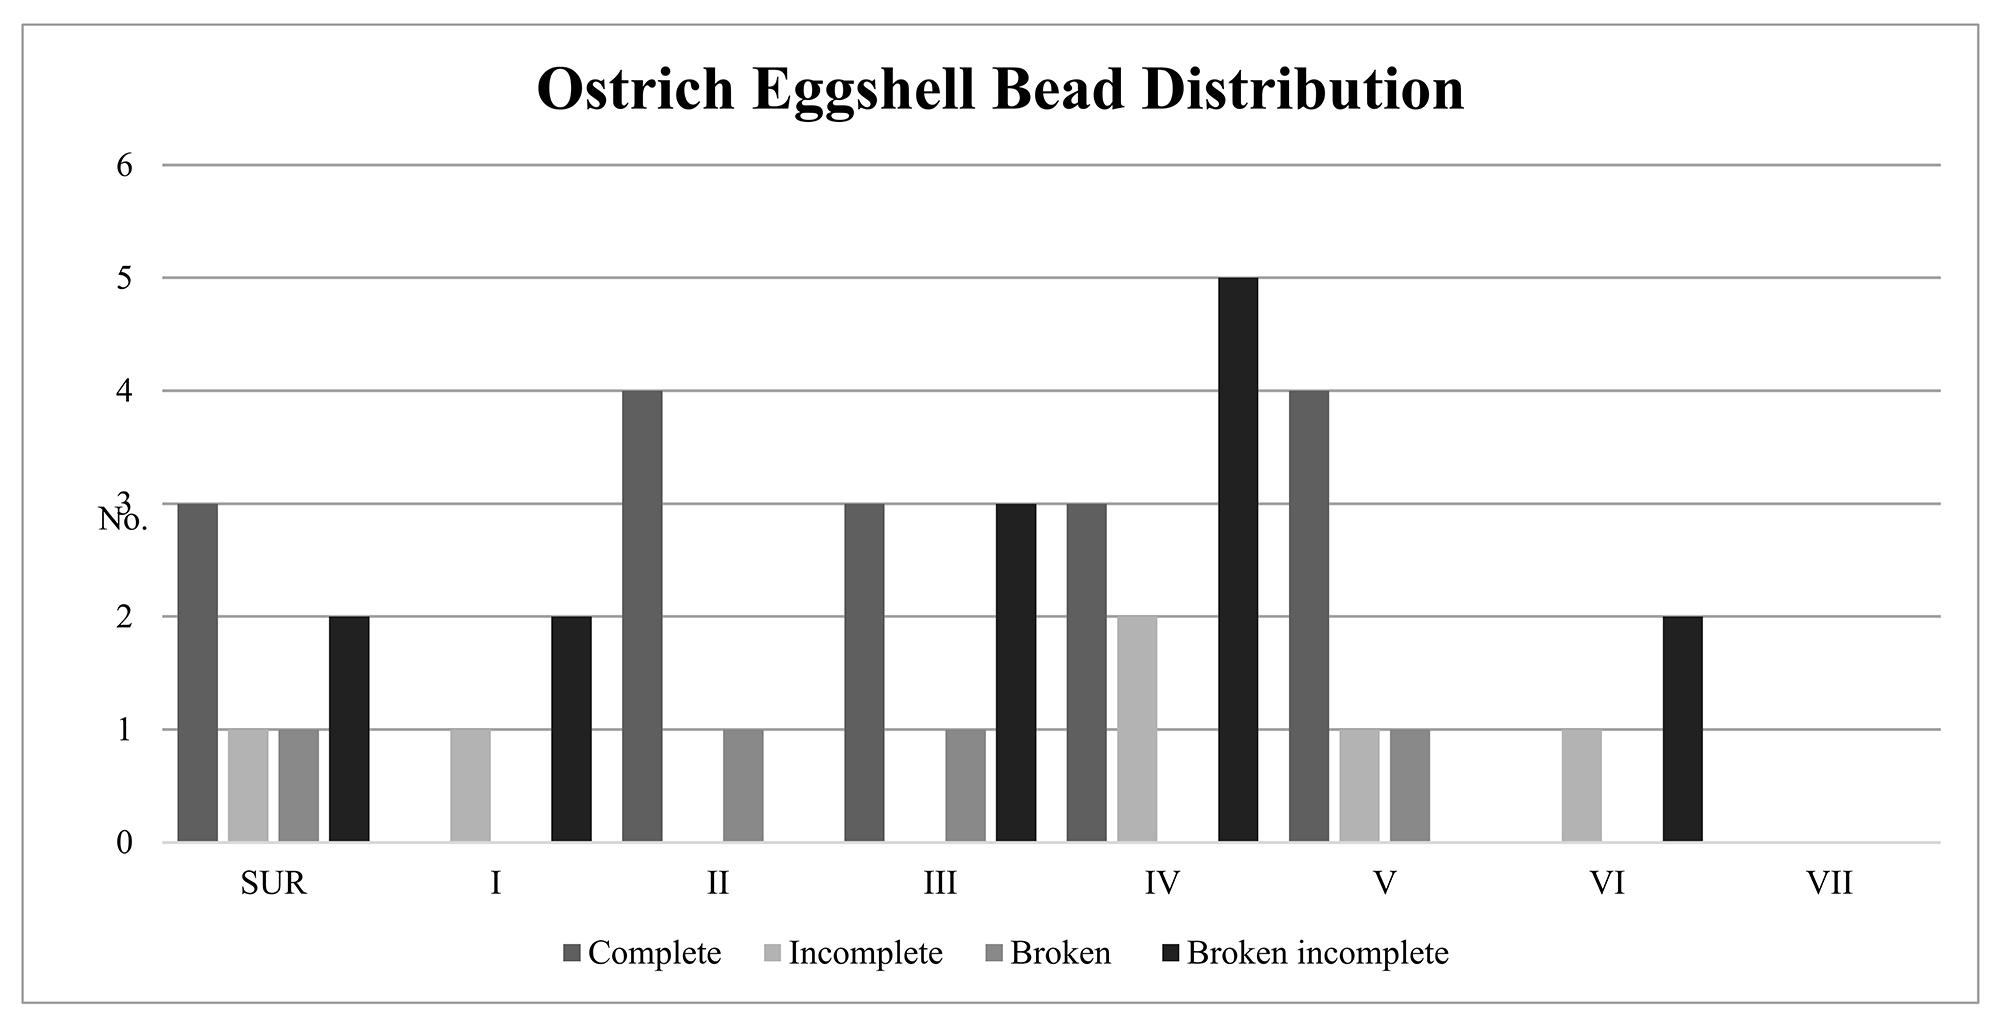
\includegraphics[width=\linewidth]{figures/Forssman-Figure09}
 		\caption{The distribution of the different ostrich eggshell bead forms is inconsistent but their presence suggests bead manufacturing was occurring at Mafunyane.}
 		\label{fig:Forssman-Figure09}
 	\end{figure}
 	
 	\begin{figure} %Figure 10
 		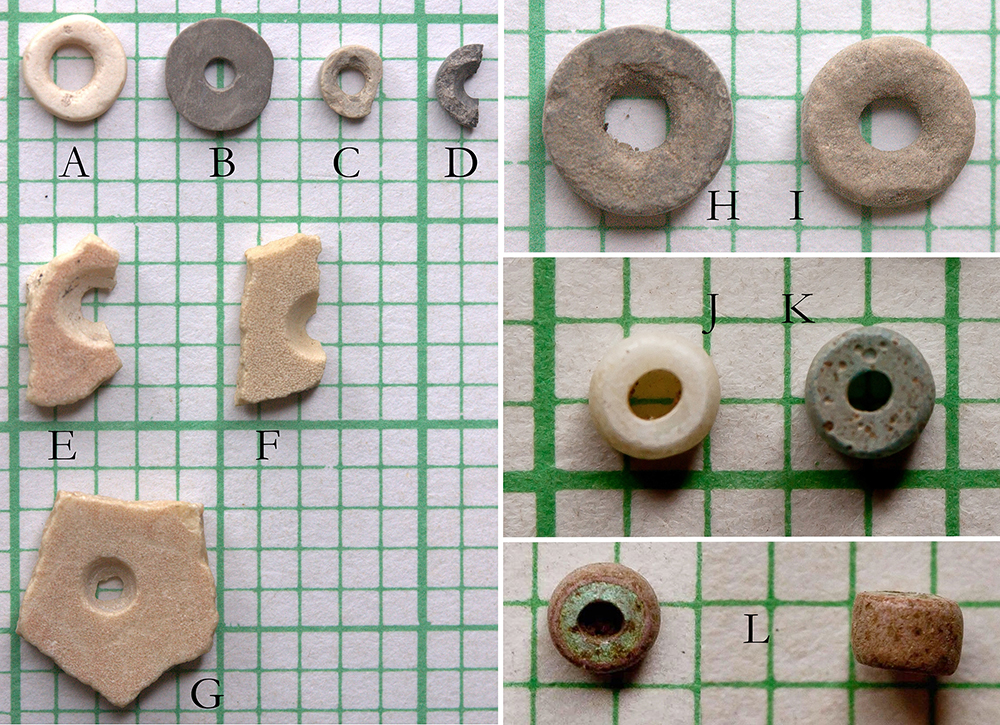
\includegraphics[width=\linewidth]{figures/Forssman-Figure10}
 		\caption{Ostrich eggshell and glass beads: A-C, H \& I, complete; D, broken complete; E-F, broken preform; and G, preform; J \& K, European possibly dating from the eighteenth century; and L, European red-on-green (\AD 1600 to 1800s; scale \SI{2}{\milli\meter}).}
 		\label{fig:Forssman-Figure10}
 	\end{figure}
 
 
 The glass beads are European, two possibly dating to the eighteenth and nineteenth centuries (\cref{fig:Forssman-Figure10}J \& K) 
 and one post-dating the seventeenth century (\cref{fig:Forssman-Figure10}L). 
 It is possible that all were introduced after foragers abandoned the rockshelter. 
 Each glass bead was given a Munsell value using the Munsell colour chart for glass beads: 
 \cref{fig:Forssman-Figure10}J is white (N9) and \cref{fig:Forssman-Figure10}K is medium blue (5.0B 4/6) 
 and each is opaque-translucent 
 \parencite[slight glow of light along edges;][70]{Wood_2011}. 
 \Cref{fig:Forssman-Figure10}L is opaque with an outer colour of orchid mist (2.5RP 7/4) and an inner colour of light turquoise (10.0GB 7/4).  
 \textcite{Walker_1994} found six glass beads and all but one were in the top unit --– he did not place them into a typology or determine their Munsell value. 
 Only a single wound metal bead was recovered from Spit I but \textcite{Walker_1994} found a total of 16 at the site.

%\section*{Other Finds}

There are 14 pieces \marginnote{Other Finds} of worked metal, including the metal bead, between Spits I and IV (\cref{fig:Forssman-Figure11}). \textcite{Walker_1994} 
suggested that the metal he found was copper because it appears consistent with copper artefacts in the \textcites{Miller_2001}{Miller_2002} reports from K2 and around Mapungubwe. 
To confirm this, an X-ray fluorescence analyses was performed on three artefacts. 
It was found that \cref{fig:Forssman-Figure12}A and C were copper alloys (C194HiCu and C197HiCu) with all three samples relatively pure in copper (> \SI{98.8}{\percent}; \cref{fig:Forssman-Figure12,fig:Forssman-Table06}). 
Metal prills \parencite[see][]{Miller_2001}, 
likely copper but not tested, occurred in various densities between the surface and Spit V, totalling \SI{134.2}{\gram}, 
but were concentrated between Spits II and V. Also found at these depths were the two slag pieces (Spits III and IV). 
In addition, what appears to be a fragment of a tuyère was found in Spit IV and is an item used in both smithing and smelting practices \parencites{Miller_2001}{Miller_2002}. 
Lastly, a possible clay figurine fragment was also found in Spit II and appears to include a portion of the back leg, the stomach and the rump of a mammal.

	\begin{figure} %Figure 11
		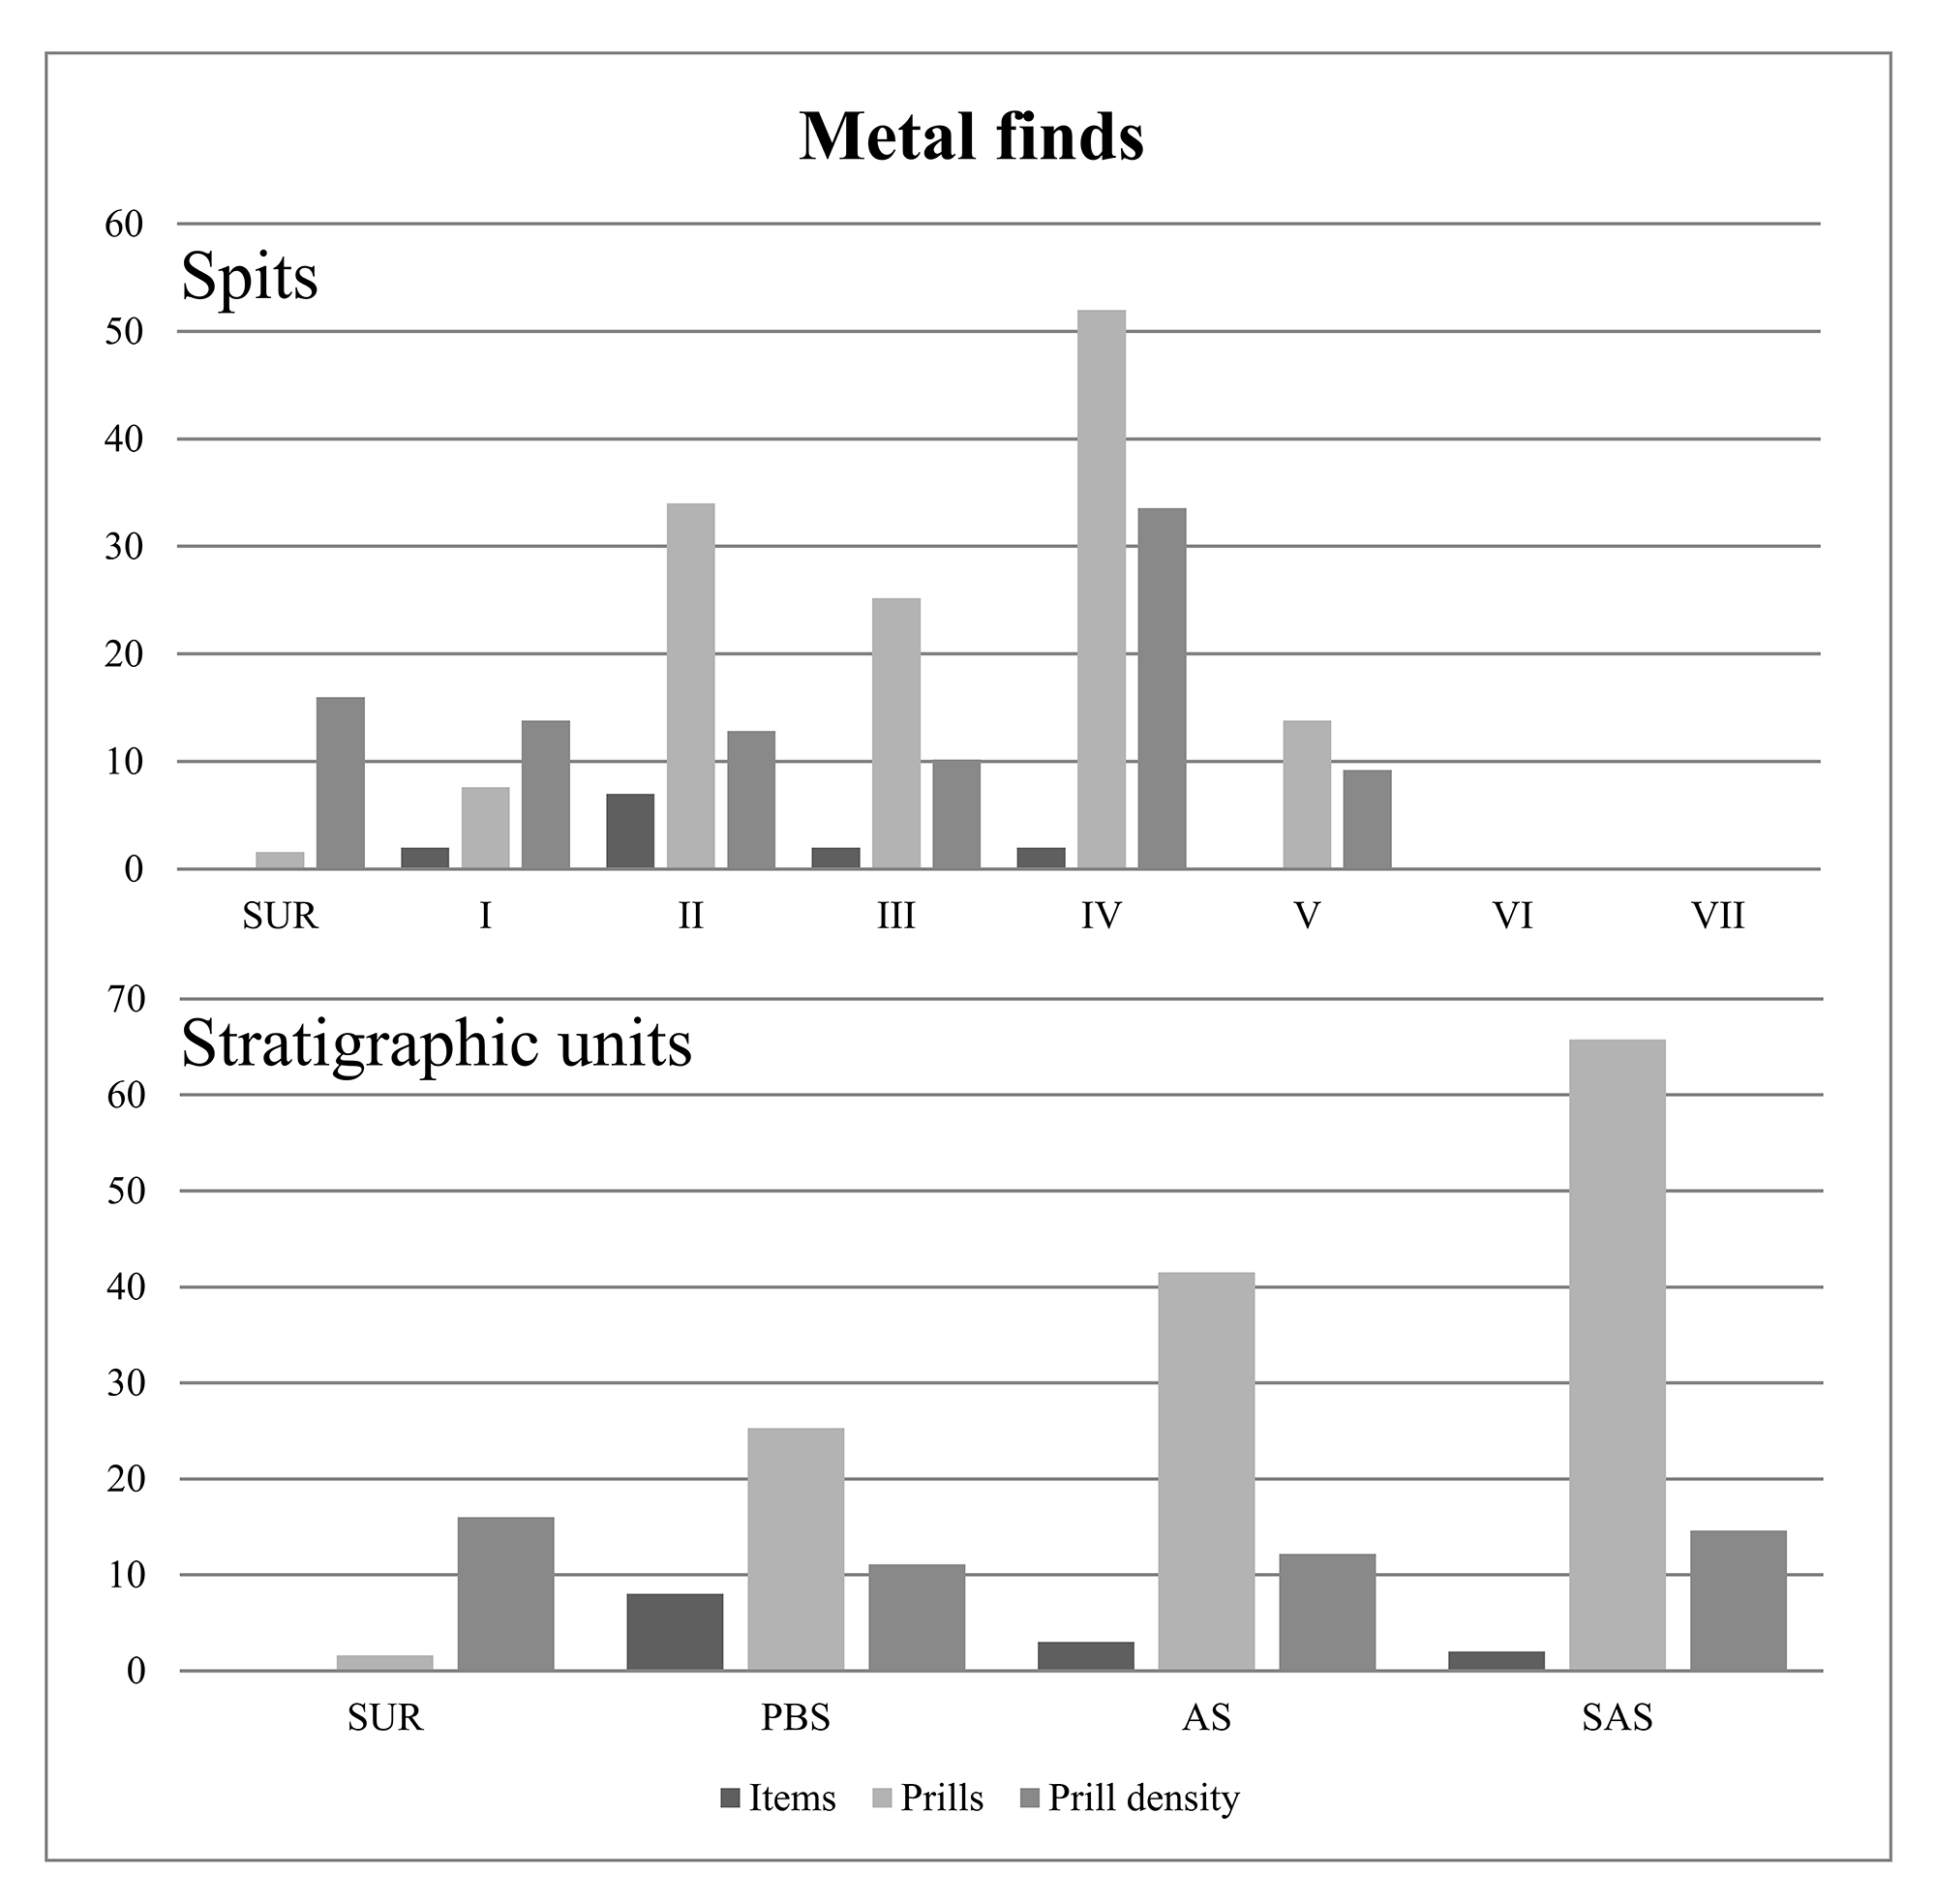
\includegraphics[width=\linewidth]{figures/Forssman-Figure11}
		\caption{The distribution of metal items, prills and the density of metal prills; metal first appears in Spit V, part of SAS.}
		\label{fig:Forssman-Figure11}
	\end{figure}

	\begin{figure} %Figure 12
		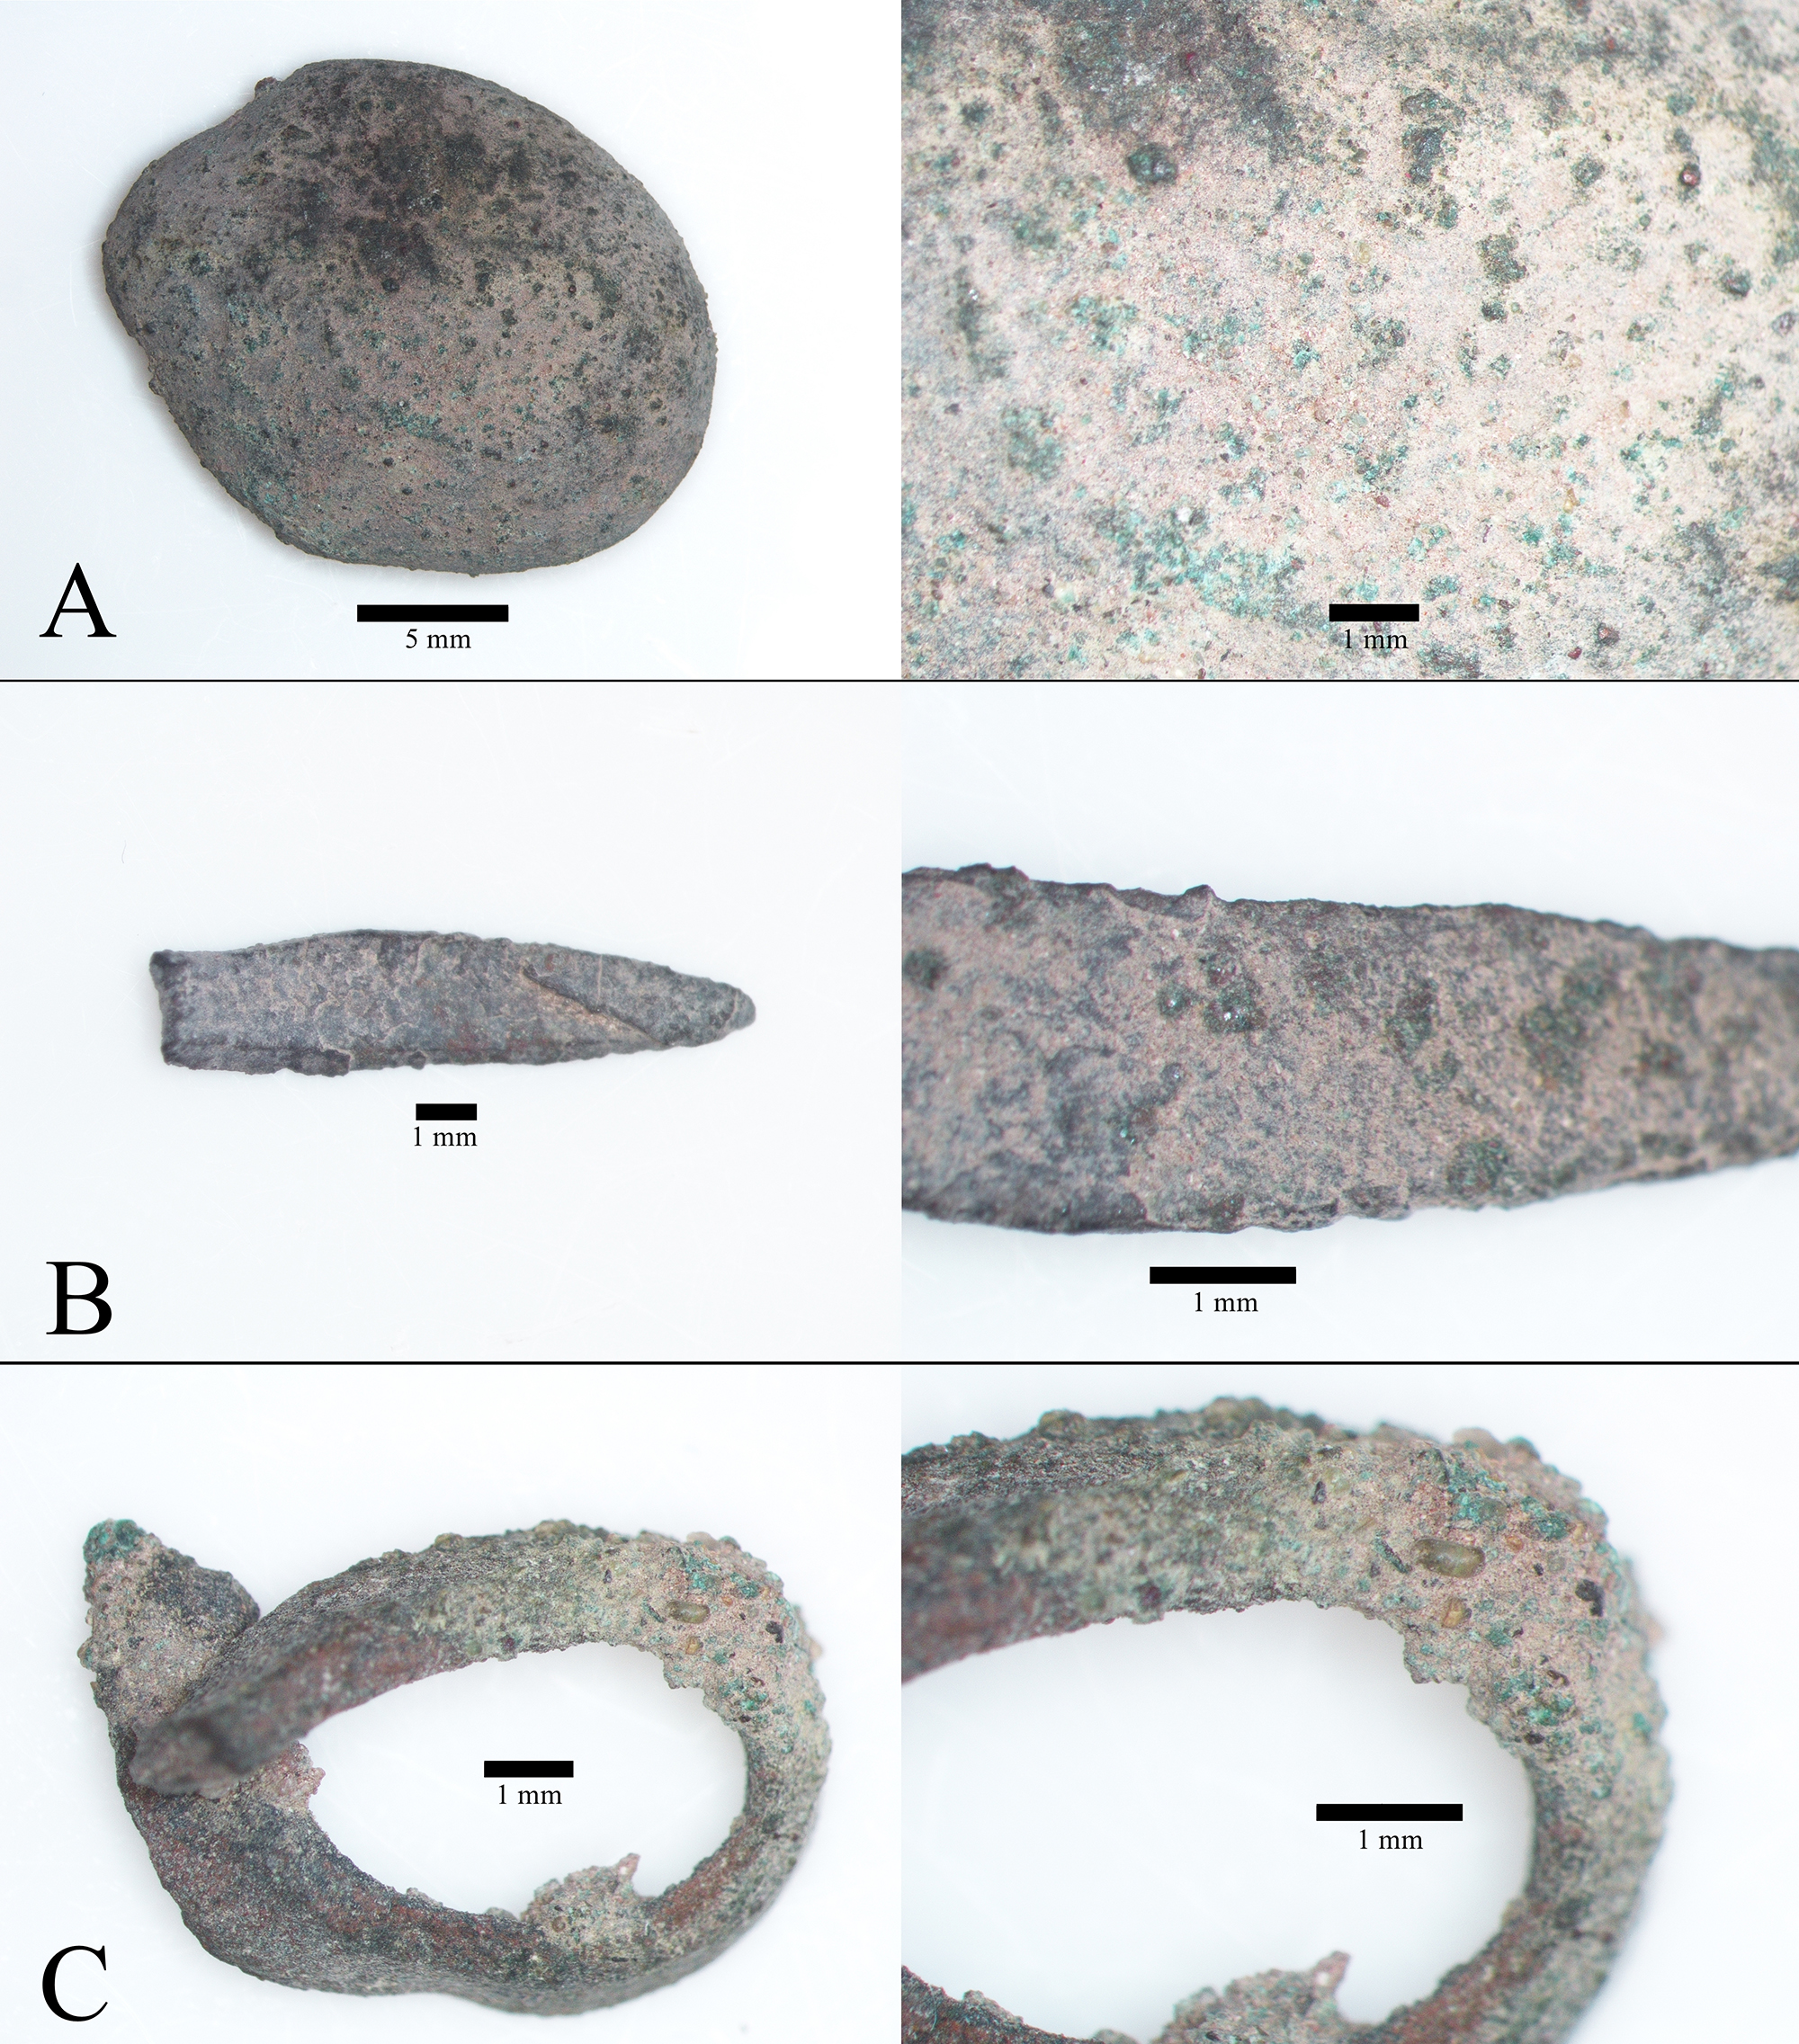
\includegraphics[width=\linewidth]{figures/Forssman-Figure12}
		\caption{The three samples submitted for XRF analysis (A – C). In each case the right imaged is a magnified portion of the sample; note the cuprous green and red patination on each specimen.}
		\label{fig:Forssman-Figure12}
	\end{figure}

    	\begin{figure} %TABLE 6
    		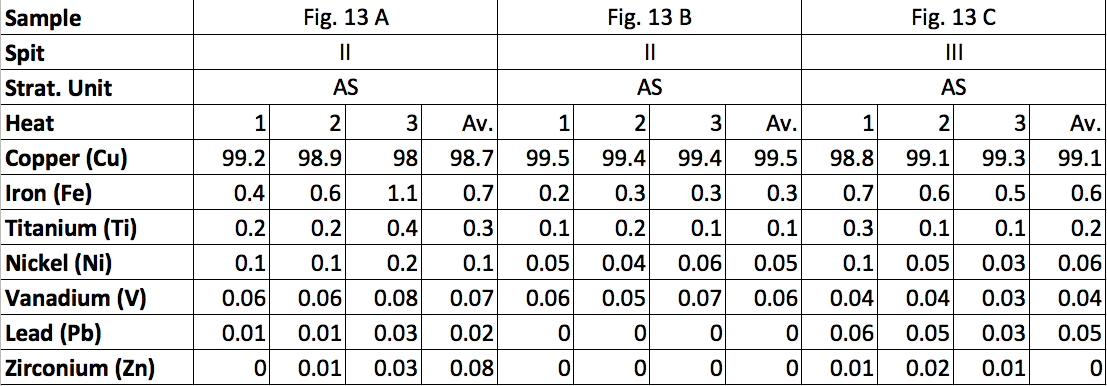
\includegraphics[width=\linewidth]{figures/Forssman-Table06}
    		\captionof{table}{XRF analysis results from samples shown in Fig 12: sample numbers in \% and Av. is the average of the three heats. Note that copper dominates and no other metal is > 1\%.}
    		\centering
    		\label{fig:Forssman-Table06}
    	\end{figure}

%\section*{Fauna}

The combined \marginnote{Fauna} mass of the faunal remains is \SI{845.8}{\gram} (\SI{82.3}{\gram}/bucket) and the highest number of identifiable specimens (NISP) 
and density of non-identified remains (\SI{300.1}{\gram}/ bucket; \cref{fig:Forssman-Table07}) occurs in Spits IV and V. 
The most frequent faunal specimen at the site is tortoise (n=50), which was mostly identified from carapace remains, followed by lizard (n=15) and small bovids (n=4). Fish remains were identified in both this and the \textcite{Walker_1994} study. 
Of interest is the presence of various items associated with farming communities but the total lack of domesticates, 
also noted by \textcite{Walker_1994}. 
It could indicate that farmers used the site for a specific and possibly non-residential purpose, that they did not have access to livestock, 
or that the food remains were deposited elsewhere. 
As will be argued, the former explanation seems most likely.

    	\begin{figure} %TABLE 7
    		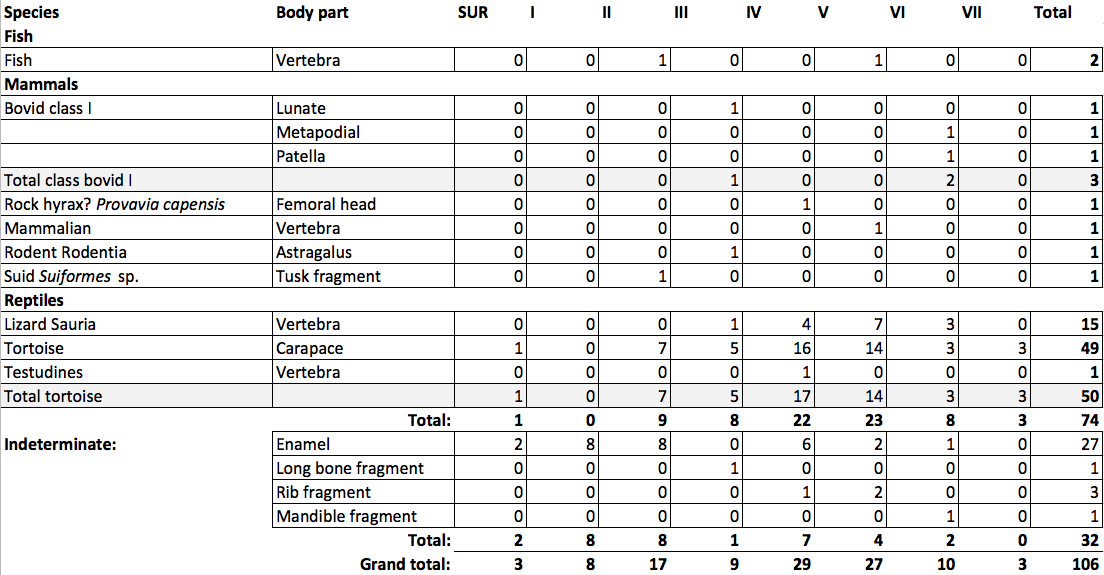
\includegraphics[width=\linewidth]{figures/Forssman-Table07}
    		\captionof{table}{The NISPs from the Mafunyane Shelter demonstrate a noticeable lack of domesticates.}
    		\centering
    		\label{fig:Forssman-Table07}
    	\end{figure}

%\section*{Rock Markings}

Grooves, cupules and \marginnote{Rock Markings} rock art were found in and around the rockshelter. Grooves were found inside on a large rock (n=21) with a cluster of more than 20 identified on an exposed rock to the west of the site. 
Nine cupules were located all occurring inside the rockshelter (\cref{fig:Forssman-Figure13}). 
The presence of metal items and ostrich eggshell beads in various stages of production might indicate that 
the grooves and cupules were used in related activities, but this cannot be said with certainty. 
Red and black monochrome rock paintings were also recorded at the site but are unfortunately heavily faded (\cref{fig:Forssman-Figure14}).
In the main portion of the rockshelter, where the excavation was performed, a black giraffe and sable or roan antelope were identified, and painted at the eastern edge are a procession of four humans, two of which appear to be females, and an indeterminate animal. 

	\begin{figure} %Figure 13
		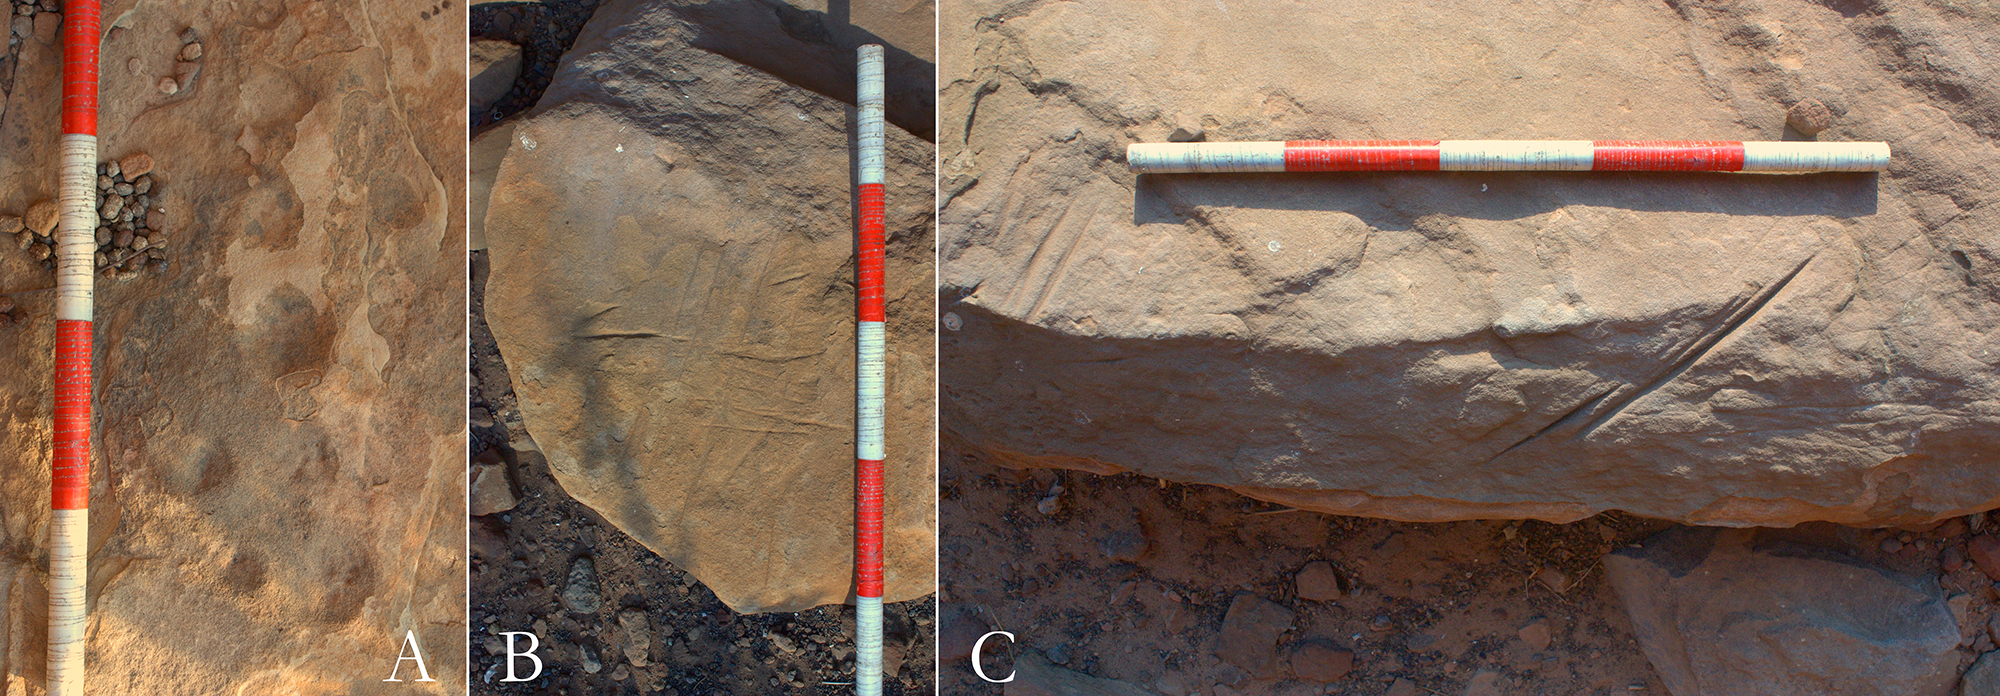
\includegraphics[width=\linewidth]{figures/Forssman-Figure13}
		\caption{Cupules (A) and grinding grooves (B \& C) from inside the rockshelter.}
		\label{fig:Forssman-Figure13}
	\end{figure}
	
	\begin{figure} %Figure 14
		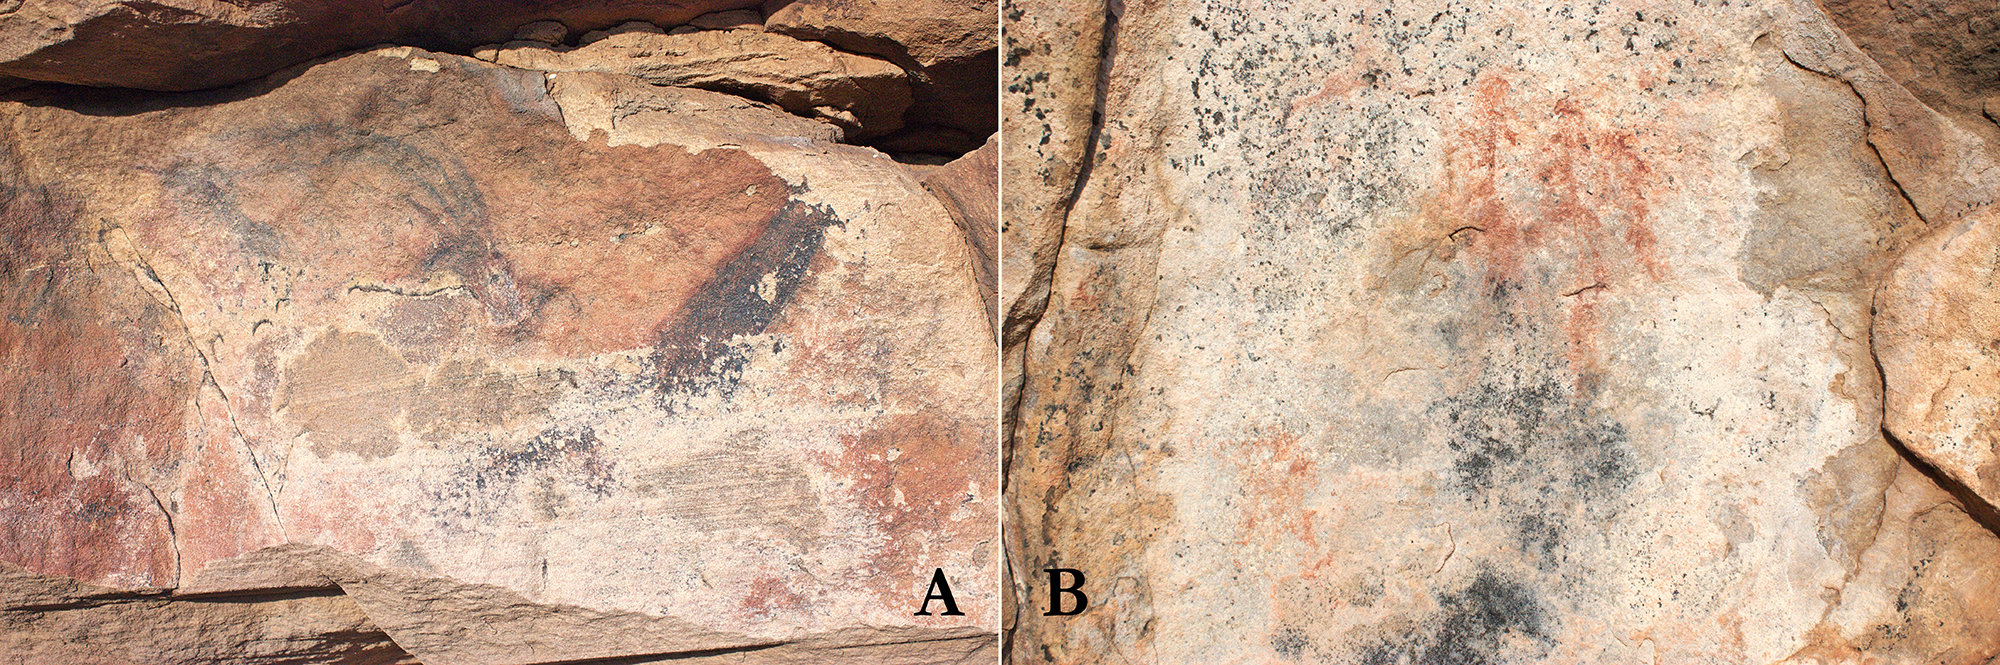
\includegraphics[width=\linewidth]{figures/Forssman-Figure14}
		\caption{Possible sable or roan antelope and giraffe (A) and a procession of four humans, two identified as female, and an indeterminate antelope (B).}
		\label{fig:Forssman-Figure14}
	\end{figure}

%\section*{Discussion and Conclusions}

Mafunyane contributes to the \marginnote{Discussion and Conclusions} growing body of work exploring the local LSA sequence. 
Until recently, most of this research was performed in South Africa and focussed primarily at large rockshelters. 
While the work of \textcite{Hall_2000} and \textcites{vanDoornum_2007}{vanDoornum_2008}{vanDoornum_2014} established a tight chronological record of the region’s LSA record as well as shifts in forager material culture, it is unlikely that by asking the same questions and excavating the same sites types we are going to further develop their findings. However, revising our research agendas and expanding our approach might lead to an improved regional understanding of LSA dynamics. Achieving this includes working in Botswana and Zimbabwe. Mafunyane, in part, contributes to these renewed goals. 

It would be remiss to not first consider the possibility of post-depositional mixing given the inverted radiocarbon dates. If this has occurred, it might explain the overturned results. The occurrence of metal-working related activities (discussed below) may have altered the deposit inadvertently. The extent of this cannot be fully assessed until further analysis is performed, but the lack of ceramics and metal in the basal level might suggest that if mixing occurred, it did not affect the entire assemblage equally. Nevertheless, the dated range is from \AD 941 to 1235, a roughly 300 year period, and if accurately identified the diagnostic ceramics appear to fall within this phase. To some extent supporting this is the dominance of scrapers in all of the stratigraphic levels, typical of contact period LSA assemblages. Since it appears that the site was occupied over a short period of time, mixing, therefore, does not preclude the possibility of interpreting the site’s use by foragers and metal-working people. However, the relationship between the site’s occupants is unknown because the exact timing of their use within the site’s occupation phase cannot be established. 

The LSA material recovered from Mafunyane is similar to what has been found at other locally excavated sites. Namely, it is dominated by CCS materials and has a variety of formal tools. The large amount of stone tools is interesting, and there is a far greater density of them than at Balerno Main Shelter, 
a local aggregation site \parencite{vanDoornum_2008}. Perhaps contributing to this is evidence of primary manufacturing at the site, suggested by the large amount of stone chips and cores. The site is located near to the Limpopo River and a seasonal stream from which cobbles could easily have been sourced. The formal tool assemblage is diverse, 
which may suggest that a variety of activities took place, but it is, as mentioned earlier, dominated by scrapers. Scraper lengths vary throughout the deposit, changing inconsistently between both the spits and stratigraphic units, whereas backed tools decrease in length into the upper levels. The inconsistent change in scraper length does not necessarily indicate mixing because the site was occupied over a short period of time and it might suggest that scraper length was not an important consideration in tool production during this period. Lastly, 
the faunal record is relatively small. This could relate to spatial dynamics or behaviour activities at the site influencing discard patterns or it might suggest Mafunyane was occupied by a small group of foragers. Represented in the faunal record is a variety of small mammals – mostly trappable – some reptiles and fish and an absence of larger animals and domesticates. In summary, there is evidence to suggest that the site was a major living camp, as \textcite{Walker_1994} concluded, but the limited faunal evidence found in both excavations may suggest otherwise.

It is difficult to interpret the farmer presence at the site because there is little evidence indicating their use or occupation. No domesticates or homestead features such as grainbin foundations, hut remains, middens or a kraal were recorded – perhaps expected in a rockshelter – and the ceramics could easily have been acquired by foragers through trade. However, in the ashy deposit were metal prills, found between the surface and Spit VI, along with metal tools and a tuyère fragment. The \textcite{Walker_1994} excavation also revealed comparable densities of these findings in addition to a clay pipe and crucible. Considering the presence of these artefacts at the site, the farmer use of Mafunyane might have been primarily for metal-working with little other activities occurring in the rockshelter. This is the only local rockshelter within which such activities have been identified and irrespective of mixing is an important finding.

The excavations at Mafunyane have assisted with our understanding of the LSA sequence in the region. Most intriguing and worthy of additional research attention is the appearance of a metal assemblage in a LSA context and what this might mean in terms of forager-farmer interactions. Additionally, establishing tighter chronological control of the site, such as by performing a refitting analysis, could help determine the degree of mixing. A large open-air courtyard in front of the rockshelter is also densely populated with LSA artefacts and although possibly disturbed, studying this area might provide greater resolution regarding the spatial dynamics of Mafunyane’s occupation. However, while the site is small and might not be revisited in future studies, it nevertheless demonstrates the complex and nuanced LSA sequence of the Greater Mapungubwe Landscape as well as the challenges facing those who study this aspect of the region’s archaeological sequence.

%\section*{Acknowledgements}
\myseparator

For \marginnote{Acknowledgements} funding, the Palaeontological Scientific Trust and Scatterlings of Africa program, the Meyerstein Fund and the South African National Research Fund are thanked along with the support given by the Mashatu Game Reserve and Tuli Safari Lodge. I thank Abigail Moffett, Ceri Ashley, Christian Louw, Lu-Marie Fraser and Peter Mitchell for commenting on an earlier draft. Abigail Moffett and Foreman Bandama are thanked for their help with the metal identification and Alexander Antonites for assistance with the ceramics. Wendy Voorvelt assisted with \cref{fig:Forssman-Figure01,fig:Forssman-Figure02,fig:Forssman-Figure03}.


%notes to self: check \num why it's doing a "." instead of a ","
%notes to self: what about personal communication citations
%notes to self: how are we coding subsections?
%notes to self: why does it get angry with my \gram code but look normal in pdf


	%----------------------------------------------------------------------------------------
	
	\printbibliography[heading=subbibliography] 
	\label{Forssman:lastpage}
%------------------------------------------------------------------------------
\closingarticle